\documentclass[conference]{IEEEtran}
\usepackage{fontspec}
\setmainfont{texgyretermes}[Extension=.otf, UprightFont=*-regular, BoldFont=*-bold,
  ItalicFont=*-italic, BoldItalicFont=*-bolditalic]
\setmonofont{DejaVuSansMono}[Extension=.ttf, BoldFont=*-Bold, Scale=0.82]
\usepackage{amsmath,amssymb}
\usepackage{tabularx,booktabs,enumitem,fancyvrb,xcolor,tikz,cite}
\usetikzlibrary{positioning,arrows.meta}
\usepackage[hidelinks]{hyperref}
\newcommand{\Tq}{T_{\mathrm{Q}}}
\newcommand{\tfix}{t_{\mathrm{fix}}}
\newcommand{\Ch}{\mathrm{Ch}}
\providecommand{\E}{}\renewcommand{\E}{\mathbb{E}}
\newcommand{\pos}[1]{\left[#1\right]^{+}}
\providecommand{\lt}{}\renewcommand{\lt}{<}
\providecommand{\gt}{}\renewcommand{\gt}{>}
\newcommand{\leantag}{\textsuperscript{\textsf{\scriptsize[Lean]}}}
\newenvironment{envblock}{\par\smallskip\noindent\ignorespaces}{\par\smallskip}
\setlist{leftmargin=*, nosep, topsep=2pt}
\begin{document}
\title{Topological Post-Quantum Cryptography Discovery\\[4pt]\large A typed graph model of harvest-now and forge-later risk, with exposure windows, break-time semantics, and remediation planning}
\author{\IEEEauthorblockN{Rick Glenn}
\IEEEauthorblockA{Technical Cofounder, Dytallix, Inc.\\
rick@dytallix.com}}
\maketitle
\begin{abstract}
Migrating an enterprise to post-quantum cryptography (PQC) requires knowing which cryptographic primitives protect which data and which trust relationships, and in what order to replace them. Endpoint-by-endpoint inventories miss a basic fact: data protected by quantum-safe cryptography on one hop can be exposed by vulnerable cryptography on another hop it later traverses. We model the estate as a typed, attributed multigraph that separates assets, data classes, channels (each carrying a stack of cryptographic layers), and trust relations. Primitives are classified by a \emph{break time}, which unifies quantum vulnerability (Shor, Grover) with classical deprecation, and composes through explicit rules for layers, nested channels, and hybrid constructions.

For the harvest-now, decrypt-later (HNDL) threat we define an \emph{exposure window}: the span of traffic that is both recordable and still sensitive when it becomes decryptable. With long transmission history it reduces exactly to Mosca's inequality. It also splits risk into a sunk part that migration cannot recover and a remediable part that it can, and it extends to a probability distribution over the arrival of a cryptographically relevant quantum computer. Trust-now, forge-later (TNFL) risk is modeled separately on the trust graph, through the time each key remains accepted by verifiers, and propagates in the opposite direction. We prove dominance, monotonicity, and condensation-equivalence properties of the propagation, machine-check the exposure-window lemma, the core risk properties, the fixpoint and condensation results, and the layer-cake identity in Lean 4, give a linear-time algorithm per lifespan tier, and show that budgeted remediation selection is NP-hard and not submodular under worst-case aggregation. Worked examples, a CycloneDX CBOM mapping, generalizations to arbitrary algorithm sunsets, and an evaluation on a reproducible testbed are included. On the testbed, run both on one host and on six cloud servers, discovery recovers the deployed configuration exactly, and a gateway that supports hybrid key exchange still negotiates classical X25519 for 26–27\% of its handshakes. Likewise, a legacy SSH client negotiates classical key exchange with a server that offers ML-KEM. We therefore extend the model to channels whose sessions negotiate a mix of configurations. Weighting exposure by the measured shares reverses which of two channels should be remediated first. On synthetic estates, propagation handles 100,000 services in under a second, rankings tolerate about 10\% error in the declared parameters but not 25\%, and the two readings choose different first fixes in about half of the estates.
\end{abstract}
\begin{IEEEkeywords}
post-quantum migration, cryptographic inventory, CBOM, Mosca inequality, attack graphs, harvest-now-decrypt-later, crypto-agility
\end{IEEEkeywords}

\section{Introduction}\label{sec:1}

A cryptographically relevant quantum computer (CRQC) would break the public-key primitives that protect most key establishment and authentication today. NIST has standardized replacements: ML-KEM (FIPS 203), ML-DSA (FIPS 204), and SLH-DSA (FIPS 205)~\cite{nist-fips203-205}, alongside the stateful hash-based signatures LMS and XMSS (SP 800-208~\cite{nist-sp800-208}). Migration timelines are now explicit: NIST IR 8547~\cite{nist-ir8547} (initial public draft) proposes deprecating quantum-vulnerable public-key algorithms at the 112-bit security level after 2030 and disallowing them after 2035, and NSA's CNSA 2.0~\cite{nsa-cnsa2} sets earlier dates for national security systems. Two threats make the problem urgent before a CRQC exists.

\begin{itemize}
\item \textbf{Harvest now, decrypt later (HNDL).} An adversary records ciphertext today and decrypts it once a CRQC is available. This applies to traffic protected by RSA key transport and equally to traffic protected by ephemeral (EC)DHE: forward secrecy protects against later compromise of long-term keys, but Shor's algorithm recovers each ephemeral shared secret directly from the recorded handshake. Forward secrecy therefore gives no protection against HNDL.
\item \textbf{Trust now, forge later (TNFL).} Once a CRQC exists, signatures under quantum-vulnerable keys can be forged. Live authentication sessions that have already ended cannot be retroactively spoofed, but any key that verifiers still accept on or after that date can be used to impersonate endpoints, issue rogue certificates, or sign malicious firmware. Long-lived signed artifacts (archives, contracts, code, ledger entries) also lose non-repudiation, because a forger can produce signatures indistinguishable from historical ones.
\end{itemize}

Cryptographic inventories that report each endpoint in isolation cannot tell whether a database whose own connections use quantum-safe key establishment is nevertheless exposed because its data is later relayed over a quantum-vulnerable channel. They also conflate two threats that propagate in opposite directions: confidentiality exposure follows data \emph{downstream} along the channels that carry it, whereas forgery exposure follows certification \emph{down from} trust anchors to everything they vouch for. This paper builds a model that keeps these distinctions explicit.

Recent work has begun to formalize parts of this problem: formal models of migration, risk propagation over asset graphs, and structured HNDL exposure measures (Section~\ref{sec:2.5}). This paper extends that line, building in particular on the formal model of cryptographic migration of Loebenberger et al.~\cite{loebenberger2024}.

\textbf{Contributions.}

\begin{itemize}
\item A typed, attributed multigraph that separates assets, data classes, channels with layered cryptographic bundles, and trust relations (Section~\ref{sec:4}).
\item Break-time semantics for primitive classification, with composition rules for components within a layer, nested layers, and hybrid constructions. The same semantics cover quantum attacks, classical deprecation deadlines, and possible breaks of post-quantum schemes (Section~\ref{sec:5}, Section~\ref{sec:6}).
\item An HNDL exposure-window measure that recovers Mosca's inequality as a special case, separates sunk from remediable risk, supports a probability distribution over the CRQC arrival time, and extends to channels whose sessions negotiate a mix of configurations (Section~\ref{sec:6}).
\item A TNFL model, separate from HNDL, based on how long each key remains accepted by verifiers and propagated downward on the trust graph (Section~\ref{sec:7}). It quantifies when authentication becomes as urgent as confidentiality, which migration guidance usually treats only qualitatively.
\item Propagation as an idempotent fixpoint, with proofs of dominance, monotonicity, condensation equivalence, and linear running time per lifespan tier (Section~\ref{sec:6.4}, Appendix B).
\item Machine-checked proofs in Lean 4 with Mathlib of Lemmas 1 and 2, Propositions 1–4 and 6–8, and Corollary 1, with Propositions 1–3 also in expectation (Appendix C). To our knowledge these are the first machine-checked results about a PQC migration risk model.
\item Complexity results for remediation selection and scheduling, with practical heuristics (Section~\ref{sec:8}), and a mapping to CycloneDX~\cite{cyclonedx16} CBOM (Section~\ref{sec:9}).
\item A reproducible testbed with declared ground truth, deployable locally or on Hetzner Cloud, and a first evaluation of discovery accuracy, the gap between supported and negotiated key exchange, and the model's risk outputs, extended to synthetic estates of up to 100,000 services (Section~\ref{sec:13}).
\end{itemize}

The framework is a decision-support model. Its outputs are only as good as the discovered graph and the supplied parameters, and Section~\ref{sec:13} reports a first evaluation on a reproducible testbed rather than a production estate.

\section{Background and related work}\label{sec:2}

\subsection{Mosca's inequality and quantum timelines}\label{sec:2.1}

Mosca observed that if $x$ is the number of years data must stay confidential, $y$ the years needed to migrate, and $z$ the years until a CRQC exists, then $x + y > z$ implies data is already at risk \cite{mosca2018} (preprint 2015). The Global Risk Institute's annual Quantum Threat Timeline Report \cite{mosca} publishes expert-elicited probability estimates for $z$, which motivates treating it as a random variable rather than a constant. Mosca's inequality concerns confidentiality; we show in Section~\ref{sec:7} that the analogous condition for signatures has a different form.

\subsection{Quantum attacks on classical primitives}\label{sec:2.2}

Shor's algorithm solves integer factorization and discrete logarithms, including over elliptic curves, in polynomial time on a fault-tolerant quantum computer \cite{shor1997}. The best known classical attacks are sub-exponential (the number field sieve) or exponential (Pollard rho on elliptic curves), so the quantum speedup is super-polynomial. Grover's algorithm gives a quadratic speedup for unstructured search \cite{grover1996}. Grover search parallelizes poorly: $P$ machines reduce wall-clock time only by a factor of $\sqrt{P}$. For this reason NIST defines its lowest PQC security category relative to AES-128 key search and continues to approve AES-128, while CNSA 2.0 requires AES-256 for national security systems. We treat the Grover margin as a policy parameter (Section~\ref{sec:5}).

\subsection{Attack graphs and risk propagation}\label{sec:2.3}

Propagating vulnerability through network dependencies is well studied in the attack-graph literature: model-checking-based generation \cite{sheyner2002}, logic-programming reachability in MulVAL \cite{ou2005}, and probabilistic risk on Bayesian attack graphs \cite{poolsappasit2012}. These works model exploitation of software vulnerabilities by an active adversary. Our setting differs in three ways: the adversary for HNDL is passive and acts across time; the vulnerability is a property of cryptographic configuration that has a time-dependent break point rather than a present exploit; and the quantity of interest is a window of exposed data rather than a reachable privilege. Our propagation is an instance of algebraic path problems over idempotent semirings \cite{carre1979,mohri2002}, which guarantees well-defined fixpoints on cyclic graphs.

\subsection{Cryptographic inventory and CBOM}\label{sec:2.4}

NIST's NCCoE project on migration to PQC (SP 1800-38~\cite{nist-sp1800-38}) describes discovery tooling and inventory practice. CycloneDX introduced a Cryptographic Bill of Materials (CBOM) in version 1.6 (2024), with cryptographic-asset components describing algorithms, protocols, certificates, and related material. These efforts focus on \emph{what} cryptography exists. This paper contributes a model of \emph{how it composes} across an estate and how to rank remediation.

\subsection{Quantitative and formal models of PQC migration}\label{sec:2.5}

Several recent works formalize parts of the problem addressed here.

\begin{itemize}
\item \textbf{Formal models of migration.} Loebenberger et al.~\cite{loebenberger2024} give a formal model of cryptographic migration and use combinatorial and probabilistic arguments to analyze its expected complexity, with numerical data and case studies. Their work is the closest formal antecedent of this paper, which extends it in three ways: confidentiality and authenticity exposure are quantified in time, layered and hybrid cryptography is composed explicitly, and remediation is ranked by risk rather than only made feasible.
\item \textbf{Graph-based risk propagation.} Hasan et al.~\cite{hasan2024} use graph-theoretic analysis of cryptographic dependencies to prioritize which systems to migrate. Erlemann, Morris, and Sathe~\cite{erlemann2026} model assets as a heterogeneous knowledge graph, propagate risk along dependencies with graph-theoretic risk functionals, and attribute exposure across cryptographic domains with Shapley values. Neither, to our knowledge, gives fixpoint semantics for cyclic dependencies or separates the harvest-now and forge-later propagation directions.
\item \textbf{Harvest-now exposure measures.} Rufino, Marcelino, and Garcia~\cite{rufino2026} derive the functional form of an HNDL compromise probability from assumptions about adversary and value-decay dynamics, and argue that additive scores cannot reproduce it. Other work fits a quantum-arrival law to published expert estimates to express the cost of delaying migration \cite{shaw2026}, embed a Monte Carlo timing-risk model based on Mosca's inequality in an enterprise-cloud transition framework \cite{gupta2026}, or extends the inequality into a multi-factor risk score, QARS \cite{grigaliunas2025}, building on the Global Risk Institute methodology \cite{mosca2017}.
\item \textbf{Confidentiality versus authentication.} Migration guidance commonly treats harvest-now decryption as the more urgent threat and signatures as a later concern. Prior work on wide-area networks separates exposure priority from migration readiness and evidence confidence when deciding which services to migrate first \cite{alam2026}. Our TNFL model quantifies when authentication becomes urgent, by measuring how long keys stay accepted and propagating forgery risk down the trust graph.
\item \textbf{Remediation selection.} Mixed-integer and QUBO formulations of budget-constrained migration with dependencies have been proposed and evaluated on synthetic inventories \cite{figueira2026}.
\item \textbf{Formal verification.} Ajith, Ibrahim, and Haroon~\cite{ajith2026} translate the communication graphs of distributed systems into Tamarin models to check the secrecy and authentication of migration paths symbolically. Machine-checked work elsewhere in PQC verifies algorithm implementations. We are not aware of machine-checked results about a migration \emph{risk} model.
\end{itemize}

We found no attack-graph or Bayesian treatment of HNDL exposure, which remains an open direction.

\section{Threat model and assumptions}\label{sec:3}

Time is measured in years from the present, $t = 0$. A CRQC becomes available at time $\Tq \ge 0$, a random variable with cumulative distribution function $F$. All Shor-vulnerable primitives are assumed to fall at the same time $\Tq$: their failures are perfectly correlated.

\begin{envblock}

\textbf{HNDL adversary.} A passive adversary who, at any time $t \le 0$ or later, can record ciphertext on a channel $e$ with intensity given by the channel's observability $O(e) \in [0,1]$. From the time a channel's cryptography breaks, the adversary can recover plaintext from every recording of it, past or future.

\textbf{TNFL adversary.} An active adversary who, from time $\Tq$, can produce valid signatures under any Shor-vulnerable key, and can deliver forged artifacts or handshakes to a verifier with reachability $A(a) \in [0,1]$.
\end{envblock}

We make the following modeling assumptions and refer to them by label.

\begin{itemize}
\item \textbf{A1 (Independent layer keys).} Nested encryption layers derive keys independently, so breaking one layer reveals nothing about another.
\item \textbf{A2 (Correct hybrids).} A hybrid key establishment is secure if either component is secure, which holds for combiners that bind both shared secrets and the transcript. Constructions without this property are classified by their weakest component.
\item \textbf{A3 (Authenticated negotiation).} Before $\Tq$, protocol negotiation is protected by classical transcript authentication (as in TLS 1.3~\cite{rescorla2018}), so an adversary cannot force a downgrade. Downgrade is therefore an active, post-$\Tq$ concern, not an HNDL concern. Fallback that endpoints accept voluntarily is captured by the negotiated-suite shares of Section~\ref{sec:6.6} and Section~\ref{sec:9}, not by this assumption.
\item \textbf{A4 (Non-zero observability floor).} Internal and air-gapped segments receive a small positive $O(e)$ rather than zero, to account for insiders, provider-side taps, and misrouted traffic.
\item \textbf{A5 (Correct implementations).} Side channels, implementation defects, and key-management failures are out of scope.
\item \textbf{A6 (PQC break time).} Standardized PQC primitives are assumed unbroken ($T = \infty$) by default. The breaks of SIKE/SIDH \cite{castryck2023} and Rainbow \cite{beullens2022} show this is an assumption, and are a reason to prefer hybrids during transition. A policy can instead give each post-quantum scheme a break time $T_{\mathrm{PQ}}$, fixed or random. Schemes that are not standardized, such as sntrup761 (Section~\ref{sec:13.8}), are natural candidates. Lemma 2 and Corollary 1 give the effect on exposure, and Section~\ref{sec:13.7} reports a sensitivity analysis.
\end{itemize}

\section{System model}\label{sec:4}

\begin{envblock}

\textbf{Definition 1 (Estate graph).} The estate is a tuple $\mathcal{G} = (V_A, \mathcal{D}, E_{\mathrm{ch}}, K, E_{\mathrm{tr}})$ where

\begin{itemize}
\item $V_A = V_{\mathrm{Net}} \cup V_{\mathrm{Dev}} \cup V_{\mathrm{Store}}$ is a set of \emph{assets}: network endpoints and services, devices (appliances, HSMs, KMS), and storage (file shares, databases, images). The subsets are disjoint; a real object with several roles is several linked assets.
\item $\mathcal{D}$ is a set of \emph{data classes}. Each $d \in \mathcal{D}$ has an origin asset $o(d) \in V_A$, a criticality $C(d) \in [0,1]$, and a confidentiality lifetime $L(d) \ge 0$ in years.
\item $E_{\mathrm{ch}}$ is a multiset of directed \emph{channels} $e = (x \to y)$ between assets, oriented in the direction data moves. A request/response connection is two channels.
\item $K$ is a set of \emph{keys} (with their certificates), and $E_{\mathrm{tr}}$ is a set of directed \emph{trust edges}: $k \to k'$ when $k$ certifies $k'$, and $k \to a$ when $k$ signs or authenticates asset or artifact $a$.
\end{itemize}
\end{envblock}

Primitives live where they act. Channel cryptography is an edge attribute, because its effect depends on which hop it protects. Keys are vertices only in the trust graph, where they have dependencies of their own.

\begin{envblock}

\textbf{Definition 2 (Cryptographic bundle and layer stack).} A \emph{layer} is a bundle $\ell = (\mathsf{kex}, \mathsf{auth}, \mathsf{cipher}, \mathsf{hash})$ naming the key establishment, peer authentication, bulk encryption, and hash or MAC of one protocol instance (a TLS session, an IPsec SA, an application-level envelope). A channel carries a stack $\Lambda(e) = (\ell_1, \dots, \ell_m)$ from outermost to innermost. An end-to-end layer spanning several hops appears in the stack of each hop it covers.
\end{envblock}

Each channel also has an observability $O(e)$, a remediation time $\tfix(e) \ge 0$ (years from now until the channel's vulnerable layers are replaced), and for each data class it carries a history $H_e(d) \ge 0$ (years it has already carried $d$ under its current configuration). We write $\Ch(d)$ for the set of channels that carry $d$; Section~\ref{sec:6.4} explains how it is labeled or inferred.
\begin{table}[!t]
\centering\footnotesize
\caption{Notation.}\label{tab:1}
\begin{tabularx}{\linewidth}{>{\raggedright\arraybackslash}X>{\raggedright\arraybackslash}X>{\raggedright\arraybackslash}X}
\toprule
\textbf{Symbol} & \textbf{Domain} & \textbf{Meaning} \\ \midrule
$C(d), C(a)$ & [0,1] & Criticality of a data class or artifact \\
$L(d)$ & years & Confidentiality lifetime (Mosca's $x$) \\
$O(e)$ & [0,1] & Observability of channel $e$ to a passive recorder \\
$H_e(d)$ & years & How long $e$ has already carried $d$ in its current configuration \\
$\tfix(e)$ & years & Time until $e$ is remediated (Mosca's $y$, per channel) \\
$T_c, T_\ell, T_e$ & years $\cup$ \{$\infty$\} & Break time of a component, layer, channel (Section~\ref{sec:5}) \\
$\Tq, F$ & years & CRQC arrival time and its CDF (Mosca's $z$) \\
$\tau(k)$ & years $\cup$ \{$\infty$\} & Time until key $k$ is no longer accepted by any verifier (Section~\ref{sec:7}) \\
$A(a)$ & [0,1] & Reachability of a verifier of $a$ by a forger \\
\bottomrule
\end{tabularx}
\end{table}

\section{Primitive classification as break times}\label{sec:5}

Instead of a categorical label per primitive, each cryptographic component $c$ is assigned a \emph{break time} $T_c \in [0, \infty]$: the time from which an adversary in our threat model can defeat it. Classification becomes a mapping into break times, and every downstream formula uses break times directly. This makes the classification part of the risk computation, so a quantum-safe configuration contributes zero risk by construction.
\begin{table*}[!t]
\centering\footnotesize
\caption{Classification. 3DES is listed as classically broken: its 64-bit block makes it vulnerable to birthday attacks today, independent of Grover.}\label{tab:2}
\begin{tabularx}{\linewidth}{>{\raggedright\arraybackslash}X>{\raggedright\arraybackslash}X>{\raggedright\arraybackslash}X>{\raggedright\arraybackslash}X}
\toprule
\textbf{Class} & \textbf{Examples} & \textbf{Break time} & \textbf{Notes} \\ \midrule
Classically broken & RSA-1024, MD5, SHA-1 signatures, RC4, export suites, 3DES (Sweet32~\cite{bhargavan2016}) & $0$ & Already deprecated or practically attackable; remediate regardless of quantum timelines \\
Shor-vulnerable & RSA (any size), finite-field DH, ECDH (X25519, P-256), ECDSA, EdDSA (Ed25519), DSA & $\Tq$ & All share one random $\Tq$ \\
Grover-reduced & AES-128, SHA-256 (preimage), HMAC-SHA-256 & $\infty$ or policy $T_s$ & $\infty$ under NIST Category 1; under CNSA 2.0 a compliance deadline $T_s$ \\
Post-quantum & ML-KEM, ML-DSA, SLH-DSA, LMS/XMSS; AES-256 & $\infty$ (A6) or $T_{\mathrm{PQ}}$ & A policy may assign a finite or random $T_{\mathrm{PQ}}$ (A6, Corollary 1) \\
Hybrid & X25519MLKEM768; composite signatures & $\max(\Tq, T_{\mathrm{PQ}})$ by rule H & See below \\
Unknown & Opaque blobs, proprietary protocols & unscored & Flagged for review; optional conservative setting $T = \Tq$ \\
\bottomrule
\end{tabularx}
\end{table*}

\begin{envblock}

\textbf{Definition 3 (Composition rules for confidentiality).}

\begin{itemize}
\item \textbf{Within a layer:} confidentiality fails if either key establishment or bulk encryption fails, so $T_\ell = \min(T_{\mathsf{kex}}, T_{\mathsf{cipher}})$. Authentication does not enter, because the HNDL adversary is passive.
\item \textbf{Nested layers (A1):} plaintext is exposed only when every layer is broken, so $T_e = \max_{\ell \in \Lambda(e)} T_\ell$.
\item \textbf{Rule H, hybrid key establishment (A2):} $T_{\mathsf{kex}} = \max(T_{\mathrm{classical}}, T_{\mathrm{PQ}})$.
\end{itemize}

\textbf{Rule H for signatures.} A composite signature that verifiers accept only when \emph{both} components verify has $T = \max$ of its components. If verifiers accept \emph{either} component, $T = \min$.
\end{envblock}

A bulk cipher alone does not determine exposure. A TLS session using AES-256-GCM over ECDHE has $T_\ell = \min(\Tq, \infty) = \Tq$, so it is HNDL-exposed. Only the full bundle determines exposure.

Sequential hops are not combined by a rule in this section. Each hop that carries a data class is a separate opportunity for recording, and Section~\ref{sec:6} aggregates over them.

\section{HNDL risk: exposure windows and propagation}\label{sec:6}

\subsection{The exposure window}\label{sec:6.1}

Fix a data class $d$ and a channel $e \in \Ch(d)$. Traffic of class $d$ sent over $e$ at time $t$ is exposed if three conditions hold. First, it was sent under the current configuration: $-H_e(d) \le t \le \tfix(e)$. Second, it can be decrypted: this happens at time $\max(t, T_e)$. Third, it is still sensitive at that time: $\max(t, T_e) \lt t + L(d)$, which for $t \lt T_e$ means $t \gt T_e - L(d)$ and for $t \ge T_e$ always holds. The set of exposed transmission times is an interval.

\begin{envblock}

\textbf{Definition 4 (Exposure window).} The exposure window of $d$ on $e$ is the length of that interval:

\[ W_e(d) \;=\; \pos{\, \tfix(e) \;-\; \max\{\, -H_e(d),\; T_e - L(d) \,\}\,} \]

Its units are years of traffic.
\end{envblock}

\begin{envblock}

\textbf{Lemma 1 (Mosca recovery and decomposition).} \leantag{}

\begin{enumerate}
\item If $H_e(d) \ge L(d) - T_e$ (the channel has carried $d$ at least since the start of the sensitive window), then $W_e(d) = \pos{L(d) + \tfix(e) - T_e}$. This is Mosca's slack $(x + y - z)^+$, and $W_e(d) \gt 0$ if and only if $x + y \gt z$.
\item Let $W^0_e(d)$ be the window if the channel were fixed immediately ($\tfix = 0$). Then $W^0_e(d) = \pos{\min\{H_e(d),\, L(d) - T_e\}}$. This is the \emph{sunk} exposure: traffic already sent that will still be sensitive when it becomes decryptable. No migration can reduce it.
\item The \emph{remediable} part is $W_e(d) - W^0_e(d) = \min\{\tfix(e),\, W_e(d)\}$.
\item If $T_e = \infty$, then $W_e(d) = W^0_e(d) = 0$.
\end{enumerate}
\end{envblock}

Part 2 makes the sunk loss precise. Any recorded traffic under a Shor-vulnerable key establishment, forward-secret or not, whose sensitivity outlasts $\Tq$ is already lost. Migration controls only the remediable part. The sunk part calls for other responses: rotating credentials that crossed the channel, reducing $L(d)$ by deleting or re-scoping data, and assuming compromise in incident planning.

Rufino, Marcelino, and Garcia~\cite{rufino2026} also model HNDL exposure, as a compromise probability whose form they derive from assumptions about adversary and value-decay dynamics. The exposure window differs in two respects: it is defined per channel, so it composes with the topology of Section~\ref{sec:6.4}, and it separates the sunk part from the remediable part. A detailed comparison of the two formulations is left for future work.

\begin{envblock}

\textbf{Lemma 2 (Windows under composition).} \leantag{} For break times $T_1, T_2 \in [0, \infty]$, with the other parameters fixed, $W(\max\{T_1, T_2\}) = \min\{W(T_1), W(T_2)\}$ and $W(\min\{T_1, T_2\}) = \max\{W(T_1), W(T_2)\}$.
\end{envblock}

By Definition 3, a hybrid key establishment and a nested layer stack are therefore never more exposed than any of their parts, and a single layer is exactly as exposed as the weaker of its key establishment and bulk cipher. This holds for every value of $T_{\mathrm{PQ}}$, not only the $\infty$ of assumption A6. A hybrid protects exactly as far as its post-quantum part outlasts $\Tq$.

\subsection{Risk of a data class}\label{sec:6.2}

\begin{envblock}

\textbf{Definition 5 (HNDL risk).} For a set of channels $S$,

\[ R_S(d) \;=\; C(d)\cdot \E_{\Tq}\!\Big[\, \max_{e \in S}\; O(e)\, W_e(d) \,\Big]. \]

The \emph{propagated} risk is $R(d) = R_{\Ch(d)}(d)$. The \emph{local} risk is $R_{\mathrm{loc}}(d) = R_{\Ch_{\mathrm{loc}}(d)}(d)$, where $\Ch_{\mathrm{loc}}(d)$ is the set of channels incident to the origin $o(d)$. The sunk risk $R^0(d)$ uses $W^0$, and the remediable risk is $R(d) - R^0(d)$.
\end{envblock}

Units are criticality-weighted years of exposed traffic. The score is a ranking quantity, not a calibrated loss. The expectation is taken outside the maximum: because all Shor-vulnerable channels share one $\Tq$, the maximum over channels must be evaluated per realization, and the expectation is a one-dimensional integral. The maximum is a worst-case aggregator. A variant that accounts for multiple recording opportunities reads $O$ as an independent recording probability and replaces only the observability term, giving $\big(1 - \prod_{e : W_e \gt 0} (1 - O(e))\big) \cdot \max_e W_e(d)$ inside the expectation. It keeps the units of years.

An asset's roll-up score is $R(u) = \max\{R(d) : o(d) = u\}$, combined with its TNFL score from Section~\ref{sec:7} when a single number per asset is required.

\subsection{Properties}\label{sec:6.3}

\begin{envblock}

\textbf{Proposition 1 (Dominance).} \leantag{} $R(d) \ge R_{\mathrm{loc}}(d)$ for every $d$.

\textbf{Proposition 2 (Monotonicity).} \leantag{} $R(d)$ is non-decreasing in $C(d)$, $L(d)$, each $O(e)$, each $H_e(d)$, and each $\tfix(e)$; non-increasing in each $T_e$ (pointwise); and non-decreasing when a channel is added to $\Ch(d)$.

\textbf{Proposition 3 (Zero risk).} \leantag{} $R(d) = 0$ if and only if, for every $e \in \Ch(d)$, either $O(e) = 0$ or, almost surely, $T_e \ge \tfix(e) + L(d)$ or $\tfix(e) + H_e(d) = 0$. In particular, a data class carried only over channels whose every layer stack contains a post-quantum or correctly bound hybrid layer has zero HNDL risk.
\end{envblock}

Proposition 1 guarantees that considering more of the topology never lowers a score. Proposition 3 guarantees that classification drives the score: quantum-safe configurations contribute nothing. Proofs are in Appendix B.

\subsection{Computing $\Ch(d)$: labeled and inferred flows}\label{sec:6.4}

When application metadata, data-loss-prevention tags, or service-mesh policy identify which data classes a channel carries, $\Ch(d)$ is given directly and $R(d)$ is computed in $O(\sum_e |\mathcal{D}(e)|)$ time, where $\mathcal{D}(e)$ is the set of classes on $e$. This \emph{labeled} mode is the precise one.

When labels are unavailable, flows are \emph{inferred} by reachability. Channels are oriented along the read path: if service $y$ calls service $x$, the response channel $x \to y$ carries data held or relayed by $x$. The inferred set is

\[ \widehat{\Ch}(d) = \{\, e = (x \to y) \in E_{\mathrm{ch}} : x \text{ is reachable from } o(d) \,\}. \]

Inference over-approximates, $\Ch(d) \subseteq \widehat{\Ch}(d)$, provided every channel that carries $d$ is in $E_{\mathrm{ch}}$ and is oriented in the direction $d$ moves. Under that condition, Proposition 2 implies inference never under-reports risk. Read-path orientation alone does not satisfy the condition for write and replication flows. It is imprecise in two known ways. A relay that forwards only some of its inputs is treated as forwarding all of them. If both directions of every connection are added, every connected service becomes a single strongly connected component and inference degenerates to "everything reaches everything." Write paths, where callers send their own data to services, should therefore be labeled rather than inferred.

Without labels, the per-class history $H_e(d)$ is unknown, so inferred mode uses a single per-channel history $H_e$ (the age of the channel's current configuration). Then the edge value $\omega_d(e) = O(e)\,W_e(d)$, for a fixed realization of $\Tq$, depends on $d$ only through $L(d)$. The per-origin value $X(u) = \max\{\omega_d(e) : e \in \widehat{\Ch}(d)\}$ satisfies

\[ X(u) = \max\Big(\max_{e = (u \to x)} \omega_d(e),\; \max_{(u \to x)} X(x)\Big). \]

\begin{envblock}

\textbf{Proposition 4 (Fixpoint and condensation).} \leantag{} On any finite channel graph, cyclic or not, the recurrence has a least fixpoint equal to the maximum of $\omega_d$ over the channels whose tail is reachable from $u$. It is constant on each strongly connected component, and the value computed on the condensation DAG (each component's value is the maximum over its outgoing channels and its successor components) equals the fixpoint.

\textbf{Proposition 5 (Complexity).} In inferred mode with per-channel histories, if data classes are grouped into $\kappa$ lifespan tiers (classes in one tier share $L$), all inferred risks are computed in $O(\kappa(|V_A| + |E_{\mathrm{ch}}|))$ time per realization of $\Tq$, and in $O(\kappa\, q\, (|V_A| + |E_{\mathrm{ch}}|))$ time with a $q$-point quadrature over $F$.
\end{envblock}

Cycles, such as mutual calls between microservices, do not threaten termination: the recurrence takes values in a finite set and is monotone, so naive iteration terminates in at most $|V_A|$ rounds. Condensation is used for speed and for the explicit linear bound. The edge value depends on the data class only through $L(d)$, given the per-channel history assumed for inferred mode, which is why the bound is per lifespan tier rather than a single linear pass. Appendix A gives the algorithm.

\subsection{Probabilistic CRQC arrival}\label{sec:6.5}

\begin{envblock}

\textbf{Proposition 6.} \leantag{} For a single channel with $H_e(d) \ge L(d)$ and $T_e = \Tq \ge 0$, let $a = \tfix(e) + L(d)$. Then

\begin{gather*}
\E\big[W_e(d)\big] = \int_0^{a} F(s)\,ds \\
\Pr\big[W_e(d) \gt 0\big] = F(a) \\
\E\big[W^0_e(d)\big] = \int_0^{L(d)} F(s)\,ds.
\end{gather*}
\end{envblock}

This complements point-value sensitivity analysis with a quantity that weights every possible arrival time by its probability. Point values remain useful as scenario checks and are shown in Section~\ref{sec:10}. Any arrival distribution can be used for $F$: an expert-survey distribution \cite{mosca}, an arrival law fitted in closed form to such estimates \cite{shaw2026}, once expressed as a distribution function, or samples from a Monte Carlo timing model \cite{gupta2026}.

\begin{envblock}

\textbf{Corollary 1 (Post-quantum components).} \leantag{} Under the conditions of Proposition 6, let a hybrid key establishment have break time $\max(\Tq, T_{\mathrm{PQ}})$, where $T_{\mathrm{PQ}} \ge 0$ has distribution function $G$ and may equal $\infty$ with positive probability. Then

\[ \E\big[W_e(d)\big] = \int_0^{a} \Pr\big[\Tq \le s,\; T_{\mathrm{PQ}} \le s\big]\,ds, \]

which equals $\int_0^a F(s)\,G(s)\,ds$ when $\Tq$ and $T_{\mathrm{PQ}}$ are independent. Without independence it lies between $\int_0^a \pos{F(s) + G(s) - 1}\,ds$ and $\int_0^a \min\{F(s), G(s)\}\,ds$. A channel protected only by the post-quantum scheme has $\E[W_e(d)] = \int_0^a G(s)\,ds$.
\end{envblock}

Under independence, a hybrid reduces expected exposure by $\int_0^a F(1 - G)$ compared with classical key establishment, and by $\int_0^a G(1 - F)$ compared with the post-quantum scheme alone. Under A6, $G \equiv 0$ and the hybrid's exposure is zero. Independence is optimistic if both breaks could come from the same advance, such as a quantum algorithm for lattice problems. The bounds hold without it, and the upper bound is attained when the two break times are comonotone.

\subsection{Channels with mixed negotiation}\label{sec:6.6}

The sessions on one channel need not all negotiate the same configuration. A gateway that supports both hybrid and classical groups negotiates hybrid with modern clients and classical with legacy ones (Section~\ref{sec:13.3}). Definitions 4 and 5 give each channel a single break time. Applied to such a channel, that break time must be the earliest among the configurations it negotiates, which scores the channel as if every session were classical.

\begin{envblock}

\textbf{Definition 4$'$ (Session mixture).} Let $K(e)$ be the set of configurations negotiated on channel $e$, where configuration $k$ has layer-stack break time $T_{e,k}$. Let $q_e(k)$ be the share of the sessions carrying $d$ that negotiate $k$, with $\sum_k q_e(k) = 1$. Let $W_{e,k}(d)$ be the window of Definition 4 with $T_e = T_{e,k}$. The \emph{share-weighted window} is

\[ \overline{W}_e(d) \;=\; \sum_{k \in K(e)} q_e(k)\, W_{e,k}(d), \]

and the \emph{share-weighted risk} $\overline{R}_S(d)$ is Definition 5 with $\overline{W}_e$ in place of $W_e$. The sunk part $\overline{W}^0_e(d)$ is defined in the same way from $W^0_{e,k}(d)$.
\end{envblock}

The two definitions answer different questions:

\begin{itemize}
\item \textbf{Worst-case reading.} Definition 5 with $T_e = \min\{T_{e,k} : q_e(k) \gt 0\}$ asks whether \emph{any} traffic of $d$ on $e$ is exposed. It suits data classes where one exposed record is enough, such as credentials, keys and session secrets.
\item \textbf{Share-weighted reading.} $\overline{R}$ asks \emph{how much} of that traffic is exposed. It suits bulk data, such as records and telemetry.
\end{itemize}

\begin{envblock}

\textbf{Proposition 7 (Session mixtures).} \leantag{} For every realization of $\Tq$:

\begin{enumerate}[label=(\alph*)]
\item A channel that negotiates a single configuration has $\overline{W}_e(d) = W_e(d)$, so the two readings agree.
\item If every configuration except $k_0$ is never broken, then $\overline{W}_e(d) = q_e(k_0)\, W_{e,k_0}(d)$: exposure scales linearly with the share of the vulnerable configuration.
\item $\overline{R}_S(d) \le R_S(d)$, where $R_S$ uses the worst-case break time. The worst-case reading is an upper bound.
\item Propositions 1 and 2 hold for $\overline{R}$, which is also non-decreasing in each share $q_e(k)$. Hence moving sessions to a configuration that breaks earlier never lowers $\overline{R}$.
\item $\overline{R}(d) = 0$ if and only if, for every $e \in \Ch(d)$ with $O(e) \gt 0$, every configuration with $q_e(k) \gt 0$ has $W_{e,k}(d) = 0$. This is the same zero set as the worst-case reading, so Proposition 3 is unchanged.
\item Sunk and remediable parts mix linearly: $\overline{W}_e(d) - \overline{W}^0_e(d) = \sum_k q_e(k) \min\{\tfix(e), W_{e,k}(d)\}$.
\end{enumerate}
\end{envblock}

The share-weighted reading rests on three assumptions:

\begin{itemize}
\item \textbf{Uniform mixing.} Traffic of $d$ is spread over the configurations in the channel's overall proportions. If one class reaches only legacy clients, its share of the classical configuration is 1. Where request metadata identifies data classes, $q_e(k)$ should be measured per class.
\item \textbf{Stationarity.} Shares measured today are applied to the whole history $H_e(d)$. If the classical share has fallen over time, the measured share underestimates historical exposure, and the sunk part should use historical telemetry or the worst-case reading.
\item \textbf{Passive adversary.} An adversary who can force classical fallback is active and outside the HNDL threat model (Section~\ref{sec:3}). The worst-case reading covers that case.
\end{itemize}

Mixed channels also add a remediation action. Besides migrating a channel, an operator can remove its classical fallback, which drives $q_e(k_0)$ to zero at the cost of refusing legacy clients. By Proposition 7(b), that action is worth $O(e)\, q_e(k_0)\, W_{e,k_0}(d)$ on the channel, before aggregation.

\section{TNFL risk on the trust graph}\label{sec:7}

Mosca's inequality does not transfer to signatures by adding validity to migration time. A forger needs a key that some verifier still \emph{accepts} at or after $\Tq$. What matters is when the key stops being accepted, not how long data stays secret.

\begin{envblock}

\textbf{Definition 6 (Acceptance horizon).} For key $k$ with remaining certificate validity $V(k)$, migration time $T_{\mathrm{mig}}(k)$, and time $D(k)$ to distribute its replacement and distrust it at every verifier,

\begin{multline*}
\tau(k) = \min\big\{\, V(k)\ \text{if verifiers enforce expiry, else } \infty, \\
 T_{\mathrm{mig}}(k) + D(k),\;\; \Lambda(k) \,\big\},
\end{multline*}

where $\Lambda(k)$ is the remaining service life of the last verifier that trusts $k$. For anchors in read-only memory or in devices that cannot be updated, $D(k) = \infty$ and $\tau(k) = \min(V(k), \Lambda(k))$, and expiry is often not enforced.

\textbf{Definition 7 (Forgery window and TNFL risk).} The forgery window of $k$ is $S(k) = \pos{\tau(k) - T_k}$, where $T_k$ is the break time of $k$'s signature algorithm ($\Tq$ for RSA or ECDSA keys, and $T_{\mathrm{PQ}}$ for post-quantum keys when A6 is relaxed). For an asset or artifact $a$ with ancestor set $\mathrm{Anc}(a)$ in the trust graph,

\[ R_{\mathrm{T}}(a) = C(a)\, A(a)\cdot \E_{\Tq}\Big[\max_{k \in \mathrm{Anc}(a)} S(k)\Big]. \]
\end{envblock}

Two features distinguish TNFL from HNDL. First, $\tau$ combines its terms with a minimum, not a sum: an enforced short validity \emph{limits} exposure rather than adding to it. Second, risk propagates \emph{downward} along certification and signing edges, from an anchor to everything it vouches for, because forging any key on a chain allows an attacker to mint valid descendants. This is the reverse of HNDL propagation. Ancestor maxima are computed with the same condensation technique as Proposition 4, applied to the reversed trust graph, which handles cycles from cross-certification.

\textbf{Long-lived signatures.} Signed artifacts that must remain non-repudiable for $L_{\mathrm{nr}}(a)$ years after signing time $t_s$ are exposed if $t_s + L_{\mathrm{nr}}(a) \gt \Tq$, regardless of key migration, because a forger can create a convincing back-dated signature. The remedy is renewal of archival evidence with post-quantum timestamps, for example Evidence Record Syntax (RFC 4998~\cite{gondrom2007}), before $\Tq$.

\textbf{Hybrid and composite signatures.} These reduce TNFL risk only when verifiers require both components (Rule H). Verifiers that accept either component, or that keep classical-only fallback, remain exposed after $\Tq$. This is where active downgrade matters, unlike the passive HNDL setting.

\section{Remediation planning}\label{sec:8}

Scores rank assets, but migration acts on configuration units: a listener's TLS policy, a KMS key, a CA hierarchy, a library version. Let $\mathcal{P}$ be the set of such units, each with a cost $c(p)$, and let fixing $p$ set the break times of the layers or keys it controls to $\infty$ at time $\tfix(p)$.

\subsection{Threshold remediation is easy}\label{sec:8.1}

To bring every data class below a threshold $\theta$ under worst-case aggregation, every channel with $C(d)\,O(e)\,W_e(d) \gt \theta$ for some $d$ must be fixed, and the sunk risk must already be at most $\theta$. The required set is the union of these channels' units, computed in one pass. If any $R^0(d) \gt \theta$, no migration plan can meet the threshold and the report should say so.

\subsection{Budgeted selection is hard and not submodular}\label{sec:8.2}

With a budget $B$, choosing units to maximize the total weight of data classes brought below $\theta$ is a set-union knapsack problem: a class counts only when \emph{all} units covering its offending channels are chosen. The set-union knapsack problem is NP-hard \cite{goldschmidt1994}. Hardness is unsurprising given the knapsack structure, and mixed-integer and QUBO formulations of budgeted migration with dependencies already exist \cite{figueira2026}. What this section adds is a structural fact about the objective that affects which heuristics are sound.

\begin{envblock}

\textbf{Proposition 8 (Non-submodularity).} \leantag{} Under worst-case aggregation, total risk reduction is not a submodular function of the set of fixed units, so greedy selection carries no general approximation guarantee.

\textbf{Example.} Let $d$ be carried by channels $e_1, e_2$ with equal $O = 1$, $W_{e_1} = W_{e_2} = 7$, and $W^0 = 5$ on both. Fixing either one alone leaves the maximum at 7, a reduction of 0. Fixing both reduces it to 5, a reduction of 2. The marginal value of $e_2$ increases when $e_1$ is added, violating diminishing returns. \hfill$\blacksquare$
\end{envblock}

The testbed shows the same effect on measured handshakes (Section~\ref{sec:13.5}).

A practical heuristic is a \emph{group-aware greedy}. Its candidates are single units and, for each data class, the group of units whose channels carry remediable exposure for that class. Each step adds the candidate with the largest marginal risk reduction per unit of cost that still fits the budget. Groups handle the complementarity in the example. On synthetic estates the heuristic reduces, but does not remove, the gap to the optimum (Section~\ref{sec:13.9}). When the noisy-OR aggregation of Section~\ref{sec:6.2} is used, gains are better behaved, and we leave the conditions for submodularity in that setting as an open question.

\subsection{Scheduling}\label{sec:8.3}

Remediable risk grows linearly with $\tfix$ (Lemma 1). Choosing an order for units subject to precedence constraints (a load balancer must support ML-KEM before the services behind it can require it) to minimize weighted completion time generalizes single-machine weighted completion-time scheduling with precedence constraints, which is NP-hard \cite{lenstra1978}. Weighted shortest-processing-time order with precedence repair is a reasonable baseline.

\section{Discovery pipeline and CBOM output}\label{sec:9}

Populating $\mathcal{G}$ uses several sources, none of which handle secret key material.

\begin{itemize}
\item \textbf{Active probing} of TLS, SSH, and IPsec endpoints reveals what a server \emph{supports} and prefers. It does not reveal what real clients \emph{negotiate}: a server offering X25519MLKEM768 may still negotiate X25519 with most legacy clients.
\item \textbf{Passive observation} (handshake telemetry from load balancers and proxies, flow logs, eBPF sensors) measures negotiated suites. A channel that negotiates several bundles is split into sub-channels, one per bundle $s$, each carrying share $\pi_e(s)$ of the traffic. Observability and windows apply per sub-channel.
\item \textbf{Control-plane interrogation} through read-only APIs of cloud KMS, certificate managers, and load balancers yields key metadata and trust relations.
\item \textbf{Static parsing} of ASN.1/DER/PEM objects, container images, and binaries yields certificates, signature algorithms, and linked cryptographic libraries. The libraries connect the CBOM to the software bill of materials (Section~\ref{sec:11}).
\item \textbf{Asset and data catalogs} provide $C$, $L$, and data-class labels, which discovery cannot infer reliably.
\end{itemize}

Output is a CycloneDX CBOM. Algorithms, protocols, certificates, and keys map to cryptographic-asset components. CycloneDX defines no standard field for a risk score, so scores and their inputs are emitted as namespaced properties, for example \texttt{dytallix:risk:hndl}, \texttt{dytallix:risk:hndl:sunk}, \texttt{dytallix:risk:tnfl}, and \texttt{dytallix:break-time-class}. Each score is accompanied by the evidence that produced it (probe result, observed negotiation share, or catalog entry), so a reviewer can trace it back to its source.

\section{Worked examples}\label{sec:10}

\subsection{HNDL: a database behind a load balancer and gateway}\label{sec:10.1}

A database $u$ holds data class $d$ with $C(d) = 1$ and $L(d) = 15$. It is read by a load balancer $v$, which is called by an API gateway $w$, which serves internet clients $z$. The read path is $u \to v \to w \to z$.
\begin{figure*}[!t]
\centering
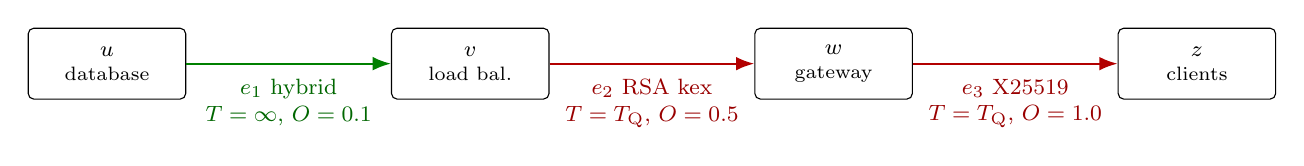
\begin{tikzpicture}[node distance=2.6cm, every node/.style={font=\footnotesize},
  box/.style={draw, rounded corners=2pt, minimum width=2.0cm, minimum height=0.9cm, align=center},
  ok/.style={-{Latex}, thick, draw=green!50!black}, bad/.style={-{Latex}, thick, draw=red!70!black}]
\node[box] (u) {$u$\\[-1pt]{\scriptsize database}};
\node[box, right=of u] (v) {$v$\\[-1pt]{\scriptsize load bal.}};
\node[box, right=of v] (w) {$w$\\[-1pt]{\scriptsize gateway}};
\node[box, right=of w] (z) {$z$\\[-1pt]{\scriptsize clients}};
\draw[ok] (u) -- node[below=2pt, align=center, text=green!40!black]{$e_1$ hybrid\\ $T=\infty$, $O=0.1$} (v);
\draw[bad] (v) -- node[below=2pt, align=center, text=red!60!black]{$e_2$ RSA kex\\ $T=T_{\mathrm{Q}}$, $O=0.5$} (w);
\draw[bad] (w) -- node[below=2pt, align=center, text=red!60!black]{$e_3$ X25519\\ $T=T_{\mathrm{Q}}$, $O=1.0$} (z);
\end{tikzpicture}
\caption{Read path for data class $d$. Green: quantum-safe channel. Red: Shor-vulnerable key establishment.}\label{fig:1}
\end{figure*}

\begin{itemize}
\item $e_1 = u \to v$: TLS 1.3 with X25519MLKEM768 and AES-256-GCM. By Rule H, $T_{e_1} = \infty$. Internal segment, $O = 0.1$.
\item $e_2 = v \to w$: TLS 1.2 with RSA key transport. $T_{e_2} = \Tq$. Shared cloud segment, $O = 0.5$.
\item $e_3 = w \to z$: TLS 1.3 with X25519 and AES-128-GCM. The key establishment gives $T_{e_3} = \Tq$; AES-128 does not change this under either Grover policy. Internet, $O = 1$.
\item $\tfix = 2$ for $e_2$ and $e_3$; both have carried $d$ for longer than $L$.
\end{itemize}

\textbf{Point scenario, $\Tq = 10$.} $W_{e_1} = 0$. For $e_2$ and $e_3$, Lemma 1 gives $W = (15 + 2 - 10)^+ = 7$, with sunk part $W^0 = \min(H, 15 - 10) = 5$ and remediable part $\min(2, 7) = 2$.

\begin{itemize}
\item Local risk: only $e_1$ is incident to $u$, so $R_{\mathrm{loc}}(d) = 1 \cdot 0.1 \cdot 0 = 0$. Local risk is zero because the database's own link is quantum-safe; an endpoint-only inventory would rate this asset as safe.
\item Propagated risk: $R(d) = \max(0.1 \cdot 0,\; 0.5 \cdot 7,\; 1.0 \cdot 7) = 7.0$.
\item Sunk risk: $R^0(d) = \max(0.5 \cdot 5,\; 1.0 \cdot 5) = 5.0$. Remediable risk: $2.0$.
\end{itemize}

Five of the seven criticality-weighted years are already lost: traffic recorded over the past five years will still be sensitive when $\Tq = 10$ arrives. Migration can prevent only the remaining two.
\begin{table*}[!t]
\centering\footnotesize
\caption{Scenario sensitivity. $e_3$ dominates the maximum in every row. Risk falls one-for-one with $\Tq$ until the sunk part vanishes at $\Tq = L = 15$; the remediable part stays at $\tfix = 2$ until $\Tq$ exceeds 15.}\label{tab:3}
\begin{tabularx}{\linewidth}{>{\raggedleft\arraybackslash}X>{\raggedleft\arraybackslash}X>{\raggedleft\arraybackslash}X>{\raggedleft\arraybackslash}X>{\raggedleft\arraybackslash}X}
\toprule
\textbf{$\Tq$} & \textbf{$W_{e_3}$} & \textbf{$R(d)$} & \textbf{Sunk $R^0(d)$} & \textbf{Remediable} \\ \midrule
5 & 12 & 12.0 & 10.0 & 2.0 \\
10 & 7 & 7.0 & 5.0 & 2.0 \\
15 & 2 & 2.0 & 0.0 & 2.0 \\
17 & 0 & 0.0 & 0.0 & 0.0 \\
\bottomrule
\end{tabularx}
\end{table*}

\textbf{Probabilistic scenario.} For illustration only (not a forecast), let $\Tq \sim \mathrm{Uniform}[5, 20]$, so $F(s) = (s - 5)/15$ on that interval. Both vulnerable channels share $\Tq$ and $\tfix$, so the maximum is attained on $e_3$ for every realization. By Proposition 6 with $a = 17$:

\begin{gather*}
R(d) = \int_5^{17} \tfrac{s-5}{15}\,ds = \tfrac{144}{30} = 4.8 \\
\Pr[\text{exposed}] = F(17) = 0.8 \\
R^0(d) = \int_5^{15} \tfrac{s-5}{15}\,ds = \tfrac{100}{30} \approx 3.33.
\end{gather*}

The expected remediable risk is about 1.47. A Monte Carlo check with $10^6$ samples agrees to two decimal places.

\textbf{Remediation.} Fixing $e_3$ now changes $W_{e_3}$ to its sunk value 5, so $R = \max(0.5 \cdot 7, 1 \cdot 5) = 5$: the full remediable reduction of 2. Fixing $e_2$ alone leaves $R = 7$, a reduction of 0. Fixing both also gives 5. The internet-facing channel $e_3$ is the priority, even though $e_2$ uses the older RSA key transport: what matters is where the vulnerable channel can be recorded.

\subsection{TNFL: firmware signed under a read-only root}\label{sec:10.2}

A fleet of field devices verifies firmware against a root key $k_R$ (RSA-4096) burned into read-only memory, with no enforced expiry and a remaining fleet service life $\Lambda = 20$. The root certifies a firmware-signing key $k_F$ (ECDSA P-256) whose certificate has $V = 3$ with enforced expiry, $T_{\mathrm{mig}} = 2$, and $D = 1$. Firmware has $C = 1$ and $A = 1$. Take $\Tq = 10$.

\begin{itemize}
\item $\tau(k_F) = \min(3, 2 + 1, 20) = 3$, so $S(k_F) = (3 - 10)^+ = 0$.
\item $\tau(k_R) = \min(\infty, \infty, 20) = 20$, so $S(k_R) = 10$.
\item $R_{\mathrm{T}}(\text{firmware}) = 1 \cdot 1 \cdot \max(0, 10) = 10$. Under the uniform prior above, $\E[S(k_R)] = \int_5^{20} F = 7.5$.
\end{itemize}

The risk sits entirely in the anchor, which cannot be migrated in the field. Rotating $k_F$ does nothing. The remedies are fleet replacement, or pre-provisioning a second, hash-based anchor (LMS or XMSS) on new devices together with a verifier policy that requires it.

\section{Generalization and adjacent domains}\label{sec:11}

\subsection{From quantum day to arbitrary sunsets}\label{sec:11.1}

Nothing in Sections~\ref{sec:5}--\ref{sec:8} depends on the cause of a break. Replacing $\Tq$ with per-algorithm deadlines $T_s(c)$, whether regulatory (NIST IR 8547's 2030 deprecation and 2035 disallowance, CNSA 2.0 dates) or cryptanalytic, turns the framework into a general crypto-agility model. Classical deprecations such as SHA-1 or TLS 1.0 are the case $T_s \le 0$. Each primitive then carries its own break-time distribution, with dependence between them (all Shor-vulnerable primitives fall together; regulatory deadlines are deterministic).

\subsection{Temporal graphs}\label{sec:11.2}

A migration plan changes the graph over time. Representing configurations as a temporal graph, where each channel's stack is a piecewise-constant function of time, lets the exposure window be computed piecewise and makes "what-if" comparison of migration plans direct.

\subsection{Adjacent domains}\label{sec:11.3}

\begin{itemize}
\item \textbf{Software supply chain.} Cryptographic libraries listed in an SBOM propagate their primitives to every binary that links them, so a vulnerable library version contributes channels and keys across the estate. The same reachability machinery applies to the dependency graph.
\item \textbf{Code signing and PKI.} These are direct instances of the TNFL trust graph, including cross-certification cycles.
\item \textbf{IoT and operational technology.} Long device lifetimes and anchors that cannot be updated make $\tau$ equal to device service life, as in Section~\ref{sec:10.2}.
\item \textbf{Identity federation.} SAML and OIDC signing keys, Kerberos, and SSH certificate authorities are trust anchors whose forgery compromises every relying service.
\item \textbf{Distributed ledgers.} A public ledger is a permanent, fully observable record: $O = 1$ and $H$ equals the chain's age, so any confidential data on chain under Shor-vulnerable encryption has maximal HNDL exposure. For TNFL, spending an output or reusing an address reveals its public key, so those funds become forgeable once $\Tq$ arrives. Migration requires protocol-level changes, and dormant keys whose owners never migrate have $\tau = \infty$.
\end{itemize}

\section{Limitations}\label{sec:12}

\begin{itemize}
\item \textbf{Discovery completeness.} The model covers only the observed estate. Air-gapped segments, shadow IT, and proprietary protocols may be missing, and missing channels make risk estimates low (Proposition 2).
\item \textbf{Flow precision.} Inferred flows over-approximate (Section~\ref{sec:6.4}). Without data-class labels on write paths, scores are conservative and may misrank assets. On synthetic estates, the median overstatement ranges from none to 8.1 times, depending on how much of what they receive services forward (Section~\ref{sec:13.9}).
\item \textbf{Parameter subjectivity.} $C$, $L$, $O$, and $\tfix$ come from catalogs and expert judgment. Rankings should be checked for sensitivity to them, not only to $\Tq$. On synthetic estates, the first fix survives about 10\% error in these parameters in most cases, but not 25\% (Section~\ref{sec:13.9}).
\item \textbf{Aggregation.} The maximum ignores multiplicity of exposure; the noisy-OR variant assumes independence. Neither is a calibrated loss model.
\item \textbf{Correlated failure.} All Shor-vulnerable primitives fail together. Aggregating risk across assets as if failures were independent would understate tail risk.
\item \textbf{Opaque ciphertext.} Field-level or application-layer encryption that discovery cannot classify is left unscored and flagged for manual review rather than given a default score.
\item \textbf{Out of scope.} Implementation defects, side channels, and cryptanalytic breaks of PQC schemes are excluded except through the policy parameter of A6.
\end{itemize}

\section{Testbed evaluation}\label{sec:13}

We evaluate the discovery pipeline of Section~\ref{sec:9} and the risk model of Sections~\ref{sec:6}--\ref{sec:8} on a reproducible testbed: a small estate whose configuration is declared in advance, so discovery can be scored exactly. The goal is to check that the pipeline recovers what is deployed and that the model's outputs behave as the formal results predict on real handshakes. It does not test whether the model predicts real-world risk; Section~\ref{sec:13.10} discusses this limit.

\subsection{Setup}\label{sec:13.1}

The estate mirrors Fig.~\ref{fig:1}, extended with a second application service and a call cycle. Services are nginx 1.28 linked against OpenSSL 3.5.9, which supports ML-KEM and ML-DSA. A modern client (curl on OpenSSL 3.5) and a legacy client (curl on OpenSSL 1.1.1) send read requests through the gateway.
\begin{table*}[!t]
\centering\footnotesize
\caption{Testbed listeners. The PKI has an RSA-4096 legacy root that is never rotated. It issues an ECDSA P-256 intermediate, which issues the leaf and firmware-signing certificates. A separate ML-DSA-65 root issues the data certificate.}\label{tab:4}
\begin{tabularx}{\linewidth}{>{\raggedright\arraybackslash}X>{\raggedright\arraybackslash}X>{\raggedright\arraybackslash}X>{\raggedright\arraybackslash}X}
\toprule
\textbf{Listener} & \textbf{Declared key exchange} & \textbf{Certificate} & \textbf{Role} \\ \midrule
gw:443 & X25519MLKEM768, X25519, P-256; TLS 1.2 and 1.3 & ECDSA P-256 & Internet edge \\
lb:8443 & TLS 1.2, RSA key transport only & RSA-2048 & Internal load balancer \\
appa:9443 & X25519 only, mutual TLS & ECDSA P-256 & Application service \\
appb:9444 & X25519 only, mutual TLS & ECDSA P-256 & Holds \emph{profile}; calls back into appa (cycle) \\
data:7443 & X25519MLKEM768 only & ML-DSA-65 & Holds \emph{records} \\
\bottomrule
\end{tabularx}
\end{table*}

Two data classes are declared: \emph{records} (origin data, $C = 1$, $L = 15$) and \emph{profile} (origin appb, $C = 0.6$, $L = 8$). Observability is 1.0 for the internet hop, 0.5 for gateway to load balancer, 0.3 for load balancer to application, and 0.1 for the remaining internal hops. Remediation times are $\tfix = 1$ for the edge and 2 elsewhere, and every channel has history $H = 20$. These parameters are declared inputs, not measurements. Trust parameters follow Section~\ref{sec:10.2}: the legacy root has non-updatable verifiers with $\Lambda = 20$, and the intermediate and firmware signer enforce expiry, with $\tau = 3$.

In each run, the modern client sends a request every second and the legacy client every 3 seconds. An active probe then runs from a separate vantage point. Telemetry comes from server access logs, which record the negotiated protocol, cipher and group, and from packet captures on every host. Discovery uses only handshakes and certificates; it never reads private keys or the declared configuration. We report three runs:

\begin{itemize}
\item \textbf{Local.} Docker on a single host, 120-second traffic window.
\item \textbf{Cloud.} Six Hetzner Cloud servers (2 vCPU, Ubuntu 24.04), 15-minute traffic window. The five estate services each run on their own server and communicate over a private network. The clients reach the gateway over its public address, and a firewall admits only the client server. The probe runs from the client server's private address. Each host captures traffic on its own interfaces, and SSH key exchange is also probed.
\item \textbf{Local with an SSH plane.} The local configuration, 120-second window, plus an SSH plane. The data service runs an SSH server, and backups of the \emph{records} data are pulled over SSH by appb (OpenSSH 10.0) and by a legacy operations host (OpenSSH 8.6). This run reproduced every TLS-plane score of the first local run exactly.
\end{itemize}

\subsection{Discovery accuracy}\label{sec:13.2}

In both runs, across the five listeners, the probe recovered TLS versions, TLS 1.3 key-exchange groups, and TLS 1.2 cipher suites with precision 1.0 and recall 1.0 against the declared configuration. It identified the key and signature algorithms of all 5 served certificates and all 10 certificates in the artifact store, including the ML-DSA-65 root and leaf. From the CMS-signed firmware it extracted the signature algorithm (ECDSA with SHA-256) and the embedded signer chain. The estate is small and deliberately discoverable, so this result validates the pipeline rather than estimating recall in a real estate.

The third run also enumerated TLS 1.2 ECDHE groups, with precision and recall 1.0: X25519 and P-256 on the gateway, none on the RSA-only load balancer. Doing this correctly needs care. In TLS 1.2, the client's supported-groups list also restricts the curves it accepts for an ECDSA certificate (RFC 8422). A probe that offers X25519 alone therefore fails against the gateway's P-256 certificate, although the server supports X25519 for key exchange. Our first probe made exactly this mistake and reported recall 0.5. The corrected probe offers each candidate group first and the certificate's curve second, then reads which group the server used for its ephemeral key. Inventory tools that test groups one at a time will under-report in the same way.

\subsection{Supported versus negotiated}\label{sec:13.3}
\begin{table*}[!t]
\centering\footnotesize
\caption{Supported versus negotiated key exchange in the local run (120 seconds) and the cloud run (15 minutes).}\label{tab:5}
\begin{tabularx}{\linewidth}{>{\raggedright\arraybackslash}X>{\raggedright\arraybackslash}X>{\raggedright\arraybackslash}X>{\raggedright\arraybackslash}X>{\raggedleft\arraybackslash}X}
\toprule
\textbf{Listener} & \textbf{Supported (probe)} & \textbf{Negotiated (local)} & \textbf{Negotiated (cloud)} & \textbf{Handshakes (local / cloud)} \\ \midrule
gw:443 & X25519MLKEM768, X25519, P-256 & X25519MLKEM768 74\%, X25519 26\% & X25519MLKEM768 73\%, X25519 27\% & 477 / 3,291 \\
lb:8443 & TLS 1.2 RSA key transport & AES256-GCM-SHA384 (RSA) 100\% & AES256-GCM-SHA384 (RSA) 100\% & 477 / 3,291 \\
appa:9443 & X25519 & X25519 100\% & X25519 100\% & 636 / 4,388 \\
appb:9444 & X25519 & X25519 100\% & X25519 100\% & 318 / 2,194 \\
data:7443 & X25519MLKEM768 & X25519MLKEM768 100\% & X25519MLKEM768 100\% & 159 / 1,097 \\
\bottomrule
\end{tabularx}
\end{table*}

The gateway supports hybrid key exchange, yet 26\% of its handshakes in the local run and 27\% in the cloud run negotiated classical X25519, all of them from the legacy client. An inventory that records only what a server supports would classify the edge as hybrid-protected. Under the worst-case reading of Section~\ref{sec:6.6}, that edge is the dominant HNDL exposure. Under the share-weighted reading, which uses the measured 26–27\%, it is not (Sections~\ref{sec:13.4}--\ref{sec:13.5}).

Packet captures agreed with server telemetry on the negotiated groups of all six observed channels in both runs. In the cloud run that covered 14,261 captured handshakes. There, each host captured its own interfaces, and the gateway's client traffic arrived on its public address. Attributing those flows to channels required joining captures with the address inventory, mapping each public and private address to its host. Real estates need the same join wherever NAT or public addressing hides the internal identity of an endpoint.

\subsection{HNDL risk}\label{sec:13.4}
\begin{table*}[!t]
\centering\footnotesize
\caption{HNDL risk computed from negotiated handshakes with labeled flows, under the worst-case reading (Definition 5) and the share-weighted reading (Definition 4$'$). The local and cloud runs gave identical values under both readings, and inferred flows gave the same values as labeled flows.}\label{tab:6}
\begin{tabularx}{\linewidth}{>{\raggedright\arraybackslash}X>{\raggedright\arraybackslash}X>{\raggedleft\arraybackslash}X>{\raggedleft\arraybackslash}X>{\raggedleft\arraybackslash}X>{\raggedleft\arraybackslash}X>{\raggedleft\arraybackslash}X>{\raggedleft\arraybackslash}X}
\toprule
\textbf{Data class} & \textbf{Scenario} & \textbf{Local} & \textbf{Propagated} & \textbf{Sunk} & \textbf{Remediable} & \textbf{Propagated (share)} & \textbf{Sunk (share)} \\ \midrule
records & $\Tq = 5$ & 0.0 & 11.0 & 10.0 & 1.0 & 6.0 & 5.0 \\
records & $\Tq = 10$ & 0.0 & 6.0 & 5.0 & 1.0 & 3.5 & 2.5 \\
records & $\Tq = 15$ & 0.0 & 1.0 & 0.0 & 1.0 & 1.0 & 0.0 \\
records & $\Tq \sim U[5,20]$ & 0.0 & 4.07 & 3.33 & 0.73 & 2.40 & 1.67 \\
profile & $\Tq = 5$ & 0.30 & 2.40 & 1.80 & 0.60 & 1.50 & 0.90 \\
profile & $\Tq = 10$ & 0.0 & 0.0 & 0.0 & 0.0 & 0.0 & 0.0 \\
profile & $\Tq \sim U[5,20]$ & 0.05 & 0.34 & 0.18 & 0.16 & 0.25 & 0.09 \\
\bottomrule
\end{tabularx}
\end{table*}

\begin{itemize}
\item \textbf{Endpoint blindness.} The records store negotiates only hybrid key exchange, so its local risk is zero, but its data crosses three Shor-vulnerable hops. Propagated risk is 6.0 at $\Tq = 10$. This is the situation that endpoint-only inventories miss (Proposition 1).
\item \textbf{Sunk exposure dominates.} At $\Tq = 10$, 5.0 of the 6.0 is sunk. Under the uniform prior, 82\% of the expected risk (3.33 of 4.07) is traffic already recorded, which no migration can recover (Lemma 1).
\item \textbf{Lifetime matters.} Profile data, with $L = 8$, carries risk only if a CRQC arrives early: 2.4 at $\Tq = 5$ and none at $\Tq = 10$.
\item \textbf{Inference over-approximates.} Reachability inference added the appa$\leftrightarrow$appb channels created by the call cycle to the records flow, although records never traverse them. Scores were unchanged only because those channels have low observability; in general inferred flows can overstate risk (Section~\ref{sec:6.4}).
\item \textbf{Negotiation shares matter, traffic volume does not.} The cloud run carried about seven times as many handshakes as the local run, yet every score is identical under both readings. The scores depend on which configurations each channel negotiates and, in the share-weighted reading, on their shares. Both were the same in the two runs. Under the share-weighted reading, the expected propagated risk of records falls from 4.07 to 2.40, and the sunk part from 3.33 to 1.67, because 73\% of the edge's sessions are hybrid. The remediable part is unchanged at 0.73. The binding channel moves from the edge to the gateway-to-load-balancer link, all of whose sessions use RSA key transport. Both clients request every path, so the uniform-mixing assumption of Section~\ref{sec:6.6} holds by construction: each path was classical in 26.8\% of the gateway's sessions in the cloud run.
\end{itemize}

\subsection{Remediation ranking}\label{sec:13.5}
\begin{table}[!t]
\centering\footnotesize
\caption{Reduction in expected total risk (both data classes, $\Tq \sim U[5,20]$) from fixing channels immediately. Both runs gave the same values.}\label{tab:7}
\begin{tabularx}{\linewidth}{>{\raggedright\arraybackslash}X>{\raggedleft\arraybackslash}X>{\raggedleft\arraybackslash}X}
\toprule
\textbf{Channel fixed now} & \textbf{Reduction (worst case)} & \textbf{Reduction (share-weighted)} \\ \midrule
gw$\rightarrow$client (edge) & 0.68 & 0.00 \\
lb$\rightarrow$gw & 0.03 & 0.73 \\
both & 0.80 & 0.73 \\
any other channel & 0.00 & 0.00 \\
\bottomrule
\end{tabularx}
\end{table}

The two readings rank the channels in opposite orders:

\begin{itemize}
\item \textbf{Worst-case reading: the edge first.} Some records cross the edge under classical X25519, and it is the most observable channel.
\item \textbf{Share-weighted reading: the link behind the edge first.} All of the link's sessions use RSA key transport, while 73\% of the edge's sessions are already hybrid, so the link carries more exposed traffic. Fixing the edge alone gains nothing under this reading, because the link remains the maximum.
\end{itemize}

Which reading applies depends on the data class (Section~\ref{sec:6.6}): the worst case for credentials and keys, the share-weighted reading for bulk records. In Section~\ref{sec:10.1}, every channel negotiates a single configuration, and priority follows where a vulnerable channel can be recorded rather than which algorithm looks oldest. Here, with measured shares, the share-weighted reading puts the oldest configuration first, because it also carries the most exposed traffic. A ranking computed from supported configurations alone could not show this.

The joint row also shows Proposition 8 on measured data. Under the worst-case reading, fixing both channels reduces risk by 0.80, more than the 0.68 + 0.03 from fixing each alone. Ranking channels by their value when fixed alone understates the link: its marginal value rises from 0.03 to 0.12 once the edge is fixed.

\subsection{TNFL}\label{sec:13.6}

The intermediate and firmware-signing keys have acceptance horizons of 3 years, so their forgery windows are zero under the uniform prior. The RSA-4096 root has $\tau = 20$ and an expected forgery window of 7.5 years. The firmware's TNFL risk of 7.5 comes entirely from the root, which matches the analysis of Section~\ref{sec:10.2}. Both runs gave the same values.

\subsection{Sensitivity to post-quantum breaks}\label{sec:13.7}

Assumption A6 sets $T_{\mathrm{PQ}} = \infty$. Table~\ref{tab:8} replaces it with a fixed break time $T_{\mathrm{PQ}}$ for both ML-KEM and ML-DSA, keeping $\Tq \sim U[5,20]$.
\begin{table*}[!t]
\centering\footnotesize
\caption{Expected propagated HNDL risk and expected forgery window $S$ (years) as the post-quantum break time varies, for the cloud run. The local run differs only in records (share) at $T_{\mathrm{PQ}} = 10$, which is 3.45 because its classical share at the edge was 26\%.}\label{tab:8}
\begin{tabularx}{\linewidth}{>{\raggedright\arraybackslash}X>{\raggedleft\arraybackslash}X>{\raggedleft\arraybackslash}X>{\raggedleft\arraybackslash}X>{\raggedleft\arraybackslash}X>{\raggedleft\arraybackslash}X>{\raggedleft\arraybackslash}X}
\toprule
\textbf{$T_{\mathrm{PQ}}$} & \textbf{records (worst)} & \textbf{records (share)} & \textbf{profile (worst)} & \textbf{profile (share)} & \textbf{$S$(ML-DSA root)} & \textbf{$S$(RSA root)} \\ \midrule
$\infty$ (A6) & 4.07 & 2.40 & 0.34 & 0.25 & 0.0 & 7.5 \\
20 & 4.07 & 2.40 & 0.34 & 0.25 & 0.0 & 7.5 \\
15 & 4.07 & 2.40 & 0.34 & 0.25 & 5.0 & 7.5 \\
10 & 4.07 & 3.46 & 0.34 & 0.25 & 10.0 & 7.5 \\
5 & 4.07 & 4.07 & 0.34 & 0.34 & 15.0 & 7.5 \\
\bottomrule
\end{tabularx}
\end{table*}

\begin{itemize}
\item \textbf{The worst-case reading does not move.} Both flows cross channels that negotiate classical key exchange: the RSA link, and the legacy sessions at the edge. By Lemma 2, a hybrid is never more exposed than its classical part, so a post-quantum break adds HNDL exposure only where a hybrid is the only protection.
\item \textbf{The share-weighted reading does.} Expected risk for records rises from 2.40 to 3.46 at $T_{\mathrm{PQ}} = 10$. At $T_{\mathrm{PQ}} = 5$, every hybrid session breaks together with $\Tq$, and the value reaches the worst-case 4.07. The hybrid sessions at the edge lose their protection as $T_{\mathrm{PQ}}$ falls into the range of $\Tq$, as Corollary 1 predicts.
\item \textbf{The ML-DSA root becomes the largest TNFL risk.} It is a pure post-quantum signature with no enforced expiry, so $S = \pos{20 - T_{\mathrm{PQ}}}$. Below $T_{\mathrm{PQ}} = 12.5$ it overtakes the RSA root. A composite root that requires both an ML-DSA and a classical signature would break at $\max(\Tq, T_{\mathrm{PQ}})$ (Rule H). By the argument of Lemma 2, its forgery window would be no larger than either component's.
\end{itemize}

\subsection{SSH key exchange}\label{sec:13.8}

The probe enumerated the SSH key-exchange algorithms offered by all five estate servers. Every server offers the hybrid sntrup761x25519-sha512 first, followed by classical X25519, NIST-curve ECDH and finite-field Diffie–Hellman. This is the default of the distribution's OpenSSH, not a testbed choice. None of the servers offers mlkem768x25519-sha256, the hybrid based on the standardized ML-KEM, because that version of OpenSSH predates it. For migration, this means the SSH channels are offered a post-quantum hybrid, but one based on a lattice KEM that has not been standardized, while the classical options remain available to any client that does not ask for it. As with TLS, the probe records only what is offered; which algorithm is negotiated depends on each client.

The SSH plane of the third run measures negotiation directly. SSH sends its key-exchange offers (KEXINIT) unencrypted, so captures show both lists, and the negotiated algorithm is the first client algorithm the server also offers (RFC 4253, Sec.~7.1). The data server offered ML-KEM and sntrup761 hybrids, X25519 and P-256, and the probe recovered that list with precision and recall 1.0.
\begin{table*}[!t]
\centering\footnotesize
\caption{Negotiated SSH key exchange on the SSH plane, from captured KEXINIT messages. The SSH server's debug log records the same totals (24 ML-KEM, 18 X25519), but its lines carry no connection identifier, so per-channel attribution comes from the captures.}\label{tab:9}
\begin{tabularx}{\linewidth}{>{\raggedright\arraybackslash}X>{\raggedright\arraybackslash}X>{\raggedright\arraybackslash}X>{\raggedleft\arraybackslash}X}
\toprule
\textbf{Channel} & \textbf{Client} & \textbf{Negotiated key exchange} & \textbf{Connections} \\ \midrule
data$\rightarrow$appb & OpenSSH 10.0 & mlkem768x25519-sha256 (100\%) & 24 \\
data$\rightarrow$ops & OpenSSH 8.6 & curve25519-sha256 (100\%) & 18 \\
\bottomrule
\end{tabularx}
\end{table*}

The pattern of Section~\ref{sec:13.3} repeats. The server supports a standardized hybrid, but the legacy client negotiates classical key exchange on every connection. Scored as its own data class ($C = 1$, $L = 15$, with $O = 0.1$ for appb and 0.3 for the operations host), the exported records carry an expected risk of 1.69, of which 1.0 is sunk. All of it comes from the operations host's channel. Upgrading that one client, or removing classical key exchange from the server's list, recovers the remediable 0.69. The SSH plane is scored separately so that the TLS-plane results of Sections~\ref{sec:13.4}--\ref{sec:13.7} stay comparable across runs. The cloud run did not include it.

\subsection{Synthetic topologies}\label{sec:13.9}

The testbed has six channels. To test the model at scale, a generator builds layered service estates: an internet client, a gateway layer, and four further layers, in which each service calls three services below it. Callbacks into upper layers create cycles.

\begin{itemize}
\item \textbf{Channels.} Each channel is classical, hybrid, mixed (classical share drawn from 5–50\%) or, rarely, classically broken, and the internet edge is mostly mixed. Observability, remediation time and history follow tiers like the testbed's.
\item \textbf{Data classes.} Classes originate in the deepest layer and in some middle services, with lifetimes from 2 to 25 years.
\item \textbf{Flows.} A service that holds a class forwards it along each of its outgoing channels with probability $f$, and every origin forwards on at least one channel. This makes $f$ control how much of the reachable graph a class actually uses, and makes labeled flows subsets of inferred ones by construction.
\end{itemize}

Estates have 200 services unless stated. All runs are seeded and use a 201-point quantile grid for $\Tq$. On the testbed, this grid differs from the scorer's 3001-point grid by at most 0.0005.

\textbf{Validation.} Given the testbed's logs, the synthetic risk engine reproduces Tables~\ref{tab:6} and~\ref{tab:7} exactly for both runs, including the joint-fix value of 0.80. On 1,000 random graphs with up to 30 nodes and cycles, the condensation algorithm of Appendix A, naive fixpoint iteration and brute-force reachability returned identical values. These are checks of the code; Propositions 4 and 7 are proved.

\textbf{Scaling.} On random graphs with three channels per service, the algorithm of Appendix A takes 1.2 ms for 1,000 services and 0.31 s for 100,000 services and 300,000 channels (one lifespan tier and one realization of $\Tq$, Python). The log-log slope is 1.21. The algorithm is linear, so we attribute the excess over 1 to memory effects in the implementation. Naive iteration on a chain processed in adversarial order needs $|V_A|$ rounds: 0.36 s for 2,000 services against 1.5 ms for condensation, growing quadratically.
\begin{table*}[!t]
\centering\footnotesize
\caption{Inferred flows (Section~\ref{sec:6.4}) against labeled flows: precision is $|\Ch(d)| / |\widehat{\Ch}(d)|$; the ratio compares worst-case propagated risk. Each row pools 40 estates (about 2,500 data classes). Classes with zero labeled risk are excluded from the ratio, between 226 and 897 per row, for example classes whose paths are all hybrid.}\label{tab:10}
\begin{tabularx}{\linewidth}{>{\raggedright\arraybackslash}X>{\raggedright\arraybackslash}X>{\raggedleft\arraybackslash}X>{\raggedleft\arraybackslash}X>{\raggedleft\arraybackslash}X}
\toprule
\textbf{Callbacks per service} & \textbf{Forwarding $f$} & \textbf{Precision (median, IQR)} & \textbf{$R_{\text{inferred}} / R_{\text{labeled}}$ (median)} & \textbf{Ratio (90th percentile)} \\ \midrule
0 & 0.25 & 0.12 (0.06–0.24) & 3.7 & 23 \\
0 & 0.50 & 0.29 (0.18–0.48) & 2.3 & 12 \\
0 & 0.75 & 0.60 (0.44–0.78) & 1.0 & 3.7 \\
0.05 & 0.25 & 0.05 (0.03–0.14) & 4.9 & 42 \\
0.05 & 0.50 & 0.16 (0.07–0.32) & 2.9 & 23 \\
0.05 & 0.75 & 0.47 (0.27–0.67) & 1.2 & 5.4 \\
0.2 & 0.25 & 0.01 (0.01–0.03) & 8.1 & 81 \\
0.2 & 0.50 & 0.05 (0.02–0.13) & 3.4 & 39 \\
0.2 & 0.75 & 0.48 (0.24–0.61) & 1.0 & 4.8 \\
any & 1.00 & 1.00 & 1.0 & 1.0 \\
\bottomrule
\end{tabularx}
\end{table*}

\textbf{Inference.} Precision falls as services forward less of what they receive and as callbacks multiply: with callbacks from 20\% of services and $f = 0.25$, the median inferred flow is 77 times larger than the labeled one. Inference never under-reports: the smallest ratio over all data classes was exactly 1, as Section~\ref{sec:6.4} guarantees. When services forward everything, it is exact. But the median risk overstatement reaches 8.1 times, and the 90th percentile 81 times. For high-criticality classes, labels are worth the effort of obtaining them.
\begin{table*}[!t]
\centering\footnotesize
\caption{Stability of the fix-one-channel ranking (worst-case reading, $\Tq \sim U[5,20]$) over 30 estates. Noise multiplies $O$, $\tfix$, $H$ and $L$ by independent $e^{\sigma Z}$, with $O$ clipped to $[0, 1]$, and uses 5 draws per estate. Weighted $\tau$ (Vigna's) is computed over channels with a non-zero gain in either ranking, because most channels tie at zero. The priors are illustrative shapes, not fits to expert surveys.}\label{tab:11}
\begin{tabularx}{\linewidth}{>{\raggedright\arraybackslash}X>{\raggedleft\arraybackslash}X>{\raggedleft\arraybackslash}X>{\raggedleft\arraybackslash}X}
\toprule
\textbf{Change from the base setting} & \textbf{Same first fix} & \textbf{Top-5 overlap} & \textbf{Weighted $\tau$ (median)} \\ \midrule
Parameter noise $\sigma = 0.1$ & 83\% & 0.84 & 0.85 \\
Parameter noise $\sigma = 0.25$ & 57\% & 0.61 & 0.66 \\
Parameter noise $\sigma = 0.5$ & 23\% & 0.37 & 0.39 \\
Parameter noise $\sigma = 1$ & 7\% & 0.13 & $-$0.01 \\
Prior: lognormal, median 12 & 100\% & 0.97 & 0.97 \\
Prior: point mass at 10 & 90\% & 0.84 & 0.87 \\
Prior: early, $5 + \mathrm{Exp}(\text{mean } 4)$ & 77\% & 0.82 & 0.88 \\
Prior: late, $U[10,30]$ & 67\% & 0.75 & 0.79 \\
Share-weighted instead of worst-case reading & 53\% & 0.57 & 0.48 \\
\bottomrule
\end{tabularx}
\end{table*}

\textbf{Rank stability.} Three results stand out:

\begin{itemize}
\item \textbf{From 25\% upward, parameter error matters more than the prior's shape.} The first fix survives about 10\% error in the declared parameters in 83\% of cases, 25\% error in 57\%, and 50\% error in 23\%. Where parameters are known only to within about 50\%, a single ranking is not meaningful, and rankings should be reported as ranges or computed as expected gains over the parameter uncertainty.
\item \textbf{Only a late arrival changes the prior's effect much.} Changing the shape of the arrival prior matters less than parameter error, except for a late prior, which moves exposure toward long-lived data.
\item \textbf{The two readings of Section~\ref{sec:6.6} disagree often.} They choose different first fixes in 47\% of estates. The reversal of Section~\ref{sec:13.5} is not an isolated case, so choosing the reading per data class is a substantive decision.
\end{itemize}
\begin{table*}[!t]
\centering\footnotesize
\caption{Greedy and the group-aware heuristic of Section~\ref{sec:8.2} against the optimal fix set found by exhaustive search, on 150 small estates (16–24 channels), 149 of which have a positive optimum. Ratios are achieved over optimal risk reduction. With $k = 1$, both heuristics are optimal. Greedy breaks ties by larger remediable exposure, then by index. With ties broken by index alone, the worst ratio at $k = 3$ drops to 0.26.}\label{tab:12}
\begin{tabularx}{\linewidth}{>{\raggedright\arraybackslash}X>{\raggedleft\arraybackslash}X>{\raggedleft\arraybackslash}X>{\raggedleft\arraybackslash}X>{\raggedleft\arraybackslash}X}
\toprule
\textbf{Reading, budget} & \textbf{Greedy: share of instances with a gap} & \textbf{Greedy: worst ratio} & \textbf{Group-aware: share with a gap} & \textbf{Group-aware: worst ratio} \\ \midrule
worst case, $k = 2$ & 4.7\% & 0.36 & 3.4\% & 0.36 \\
worst case, $k = 3$ & 11.4\% & 0.44 & 8.7\% & 0.66 \\
share-weighted, $k = 2$ & 4.7\% & 0.36 & 4.0\% & 0.36 \\
share-weighted, $k = 3$ & 8.7\% & 0.37 & 6.7\% & 0.37 \\
\bottomrule
\end{tabularx}
\end{table*}

\textbf{Greedy against optimal.} The complementarity of Proposition 8 occurs in practice:

\begin{itemize}
\item \textbf{Greedy falls short.} Greedy selection misses the optimum in up to 11\% of instances, by as much as 64\%.
\item \textbf{The group-aware heuristic helps, but does not close the gap.} It reduces how often a shortfall occurs and the average shortfall: its mean ratio is 0.984–0.991, against 0.976–0.984 for greedy. Its worst case improves only for the worst-case reading at $k = 3$, from 0.44 to 0.66.
\item \textbf{Exhaustive search is practical when the candidate set is small.} Its cost grows as $|E|^k$, so it suits small estates, or estates pruned to the channels with remediable exposure. Otherwise, the group-aware heuristic is the better default.
\end{itemize}

\subsection{Threats to validity and next steps}\label{sec:13.10}

\begin{itemize}
\item \textbf{Construct validity.} The testbed, the synthetic generator and the model were designed by the same author. The evaluation shows that the pipeline recovers the deployed configuration and that the implementation behaves as the formal results predict, and Section~\ref{sec:13.9} shows how the model behaves on estates built from the author's assumptions. It does not show that the model's scores track real-world risk.
\item \textbf{External validity.} The estate is small, synthetic and deterministic. Observability and the other model parameters are declared, not measured. The cloud run adds separate hosts, real network segments and a public edge, but it uses the same software and traffic as the local run, so the agreement of the two runs shows that the results are reproducible, not that they generalize.
\item \textbf{Coverage.} IPsec is not exercised. SSH negotiation and TLS 1.2 groups were measured in a local run only, and the SSH plane is scored as a separate data class rather than merged into the flows of Section~\ref{sec:13.4}.
\end{itemize}

The next step is a production case study: measure observability and lifetimes where possible, and compare the model's ranking with independent expert prioritization using Kendall's $\tau$. Table~\ref{tab:11} indicates how accurately the parameters must be known for such a comparison to be informative.

The testbed's Terraform and container configuration, ground truth, probe, and scorer are released with this paper, together with the synthetic generator and experiments of Section~\ref{sec:13.9}. A local run takes about two minutes. A cloud run takes about 30 minutes plus provisioning, and costs well under one euro at hourly server rates.

\section{Conclusion}\label{sec:14}

Cryptographic risk in an enterprise is a property of how primitives compose along data flows and trust chains, not of individual endpoints. Treating classification as break times, measuring HNDL exposure as a window of recorded traffic, and modeling TNFL separately through how long keys stay accepted together give a model that reduces to Mosca's inequality where it should, distinguishes losses that are already sunk from those migration can prevent, and propagates each threat in its own direction. The propagation is well defined on cyclic graphs and runs in linear time per lifespan tier. Remediation selection is hard in general, but the model exposes the structure that practical heuristics need. A testbed evaluation, run on one host and on six cloud servers (Section~\ref{sec:13}), shows three things. Discovery recovers the deployed configuration. The model separates endpoint-safe from flow-exposed data on real handshakes. And what is negotiated, not what is supported, determines exposure, in TLS and in SSH: weighting exposure by measured negotiation shares (Section~\ref{sec:6.6}) changes which channel should be fixed first. On synthetic estates, propagation scales linearly, rankings need parameters accurate to about 10\%, and the choice between the two readings changes the first fix in about half of the estates. The next step is a production case study.

\textbf{Implementation note.} The framework informs the architecture of Dytallix's QuantumSentinel platform, which implements multi-source discovery, graph construction, classification against NIST standards, and evidence-linked CycloneDX CBOM output. Automated extraction of $L(d)$ and data-class labels remains an open engineering problem.

\section*{Declarations}

\begin{itemize}
\item \textbf{Data and code availability.} The testbed is released at https://github.com/exocognosis/PQC-topology. It contains the Terraform and container configuration, the ground truth, the probe, the scorer, the report, scores and CBOM of every run, the synthetic generator and experiments of Section~\ref{sec:13.9}, and the property tests. The Lean development of Appendix C is released with it. All runs are seeded or reproducible from the released configuration.
\item \textbf{Ethics.} All probing and generated traffic targeted only infrastructure created for this study: local containers, and servers in a dedicated Hetzner Cloud project. No third-party systems were scanned. All keys and certificates are throwaway test material.
\end{itemize}

\appendices

\section{Propagation algorithm}\label{app:A}

\begin{figure*}[!t]
\begin{Verbatim}[fontsize=\footnotesize, frame=lines]
input:  channel graph (V_A, E_ch); edge values ω(e) for one lifespan tier
        and one realization (or quadrature node) of T_Q
output: X(u) = max ω over channels whose tail is reachable from u

1. Run Tarjan's algorithm; it emits SCCs S_1 … S_r in reverse
   topological order (sinks first).
2. for i = 1 … r:
       val[S_i] ← max( { ω(e) : tail(e) ∈ S_i } ∪ {0} )
       for each channel e = (x → y) with x ∈ S_i, comp(y) ≠ S_i:
           val[S_i] ← max(val[S_i], val[comp(y)])
3. for each u: X(u) ← val[comp(u)]

TNFL ancestor maxima: run the same procedure on the reversed
trust graph with vertex values S(k).
\end{Verbatim}
\caption{Propagation over the condensation DAG (Appendix A).}\label{fig:alg}
\end{figure*}

Each vertex and edge is processed a constant number of times, giving $O(|V_A| + |E_{\mathrm{ch}}|)$ per tier and quadrature node.

\section{Proofs}\label{app:B}

\begin{envblock}

\textbf{Lemma 1.} (1) If $-H_e \le T_e - L$, the inner maximum is $T_e - L$, so $W = (\tfix + L - T_e)^+$. (2) Setting $\tfix = 0$ gives $\pos{-\max(-H, T - L)} = \pos{\min(H, L - T)}$. (3) Let $m = \max(-H, T - L)$. If $m \le 0$, then $W = \tfix - m \ge \tfix$ and $W^0 = -m$, so $W - W^0 = \tfix = \min(\tfix, W)$. If $m \gt 0$, then $W^0 = 0$ and $W = (\tfix - m)^+ \le \tfix$, so $W - W^0 = W = \min(\tfix, W)$. (4) $T_e = \infty$ makes $m = \infty$. \hfill$\blacksquare$

\textbf{Lemma 2.} $W$ is non-increasing in $T$ (Proposition 2). If $T_1 \le T_2$, then $\max\{T_1, T_2\} = T_2$ and $W(T_2) \le W(T_1)$, so $W(T_2) = \min\{W(T_1), W(T_2)\}$. The case $T_2 \le T_1$ and the statement for $\min$ are symmetric. \hfill$\blacksquare$

\textbf{Proposition 1.} $\Ch_{\mathrm{loc}}(d) \subseteq \Ch(d)$, the maximum over a superset is at least the maximum over the subset for every realization, and expectation preserves the inequality. \hfill$\blacksquare$

\textbf{Proposition 2.} $W_e(d)$ is non-decreasing in $\tfix$, $H$, and $L$ and non-increasing in $T_e$, because $\max$ and $[\cdot]^+$ are monotone. Products with non-negative $O$ and $C$, maxima, and expectations preserve monotonicity. Adding a channel enlarges the set over which the maximum is taken. \hfill$\blacksquare$

\textbf{Proposition 3.} $R(d) = 0$ if and only if $O(e)\,W_e(d) = 0$ almost surely for every $e \in \Ch(d)$. $W_e(d) = 0$ if and only if $\tfix \le \max(-H, T_e - L)$, that is, $\tfix + H = 0$ or $T_e \ge \tfix + L$. A layer stack containing a post-quantum or correctly bound hybrid layer has $T_e = \infty$ by Definition 3. \hfill$\blacksquare$

\textbf{Proposition 4.} Values lie in the finite set $\{\omega(e)\} \cup \{0\}$, ordered by $\le$, and the update is monotone, so Kleene iteration from 0 reaches the least fixpoint (Knaster–Tarski). By induction on iterations, the value at $u$ is the maximum of $\omega$ over channels whose tail is reachable from $u$; vertices in one strongly connected component reach the same set, so values agree. The condensation recurrence computes exactly this maximum, by induction in reverse topological order. \hfill$\blacksquare$

\textbf{Proposition 5.} Tarjan's algorithm~\cite{tarjan1972} and the pass of Appendix A are linear; they are repeated once per lifespan tier and quadrature node. \hfill$\blacksquare$

\textbf{Proposition 6.} With $H \ge L$, $W = (a - \Tq)^+$ by Lemma 1 for every $\Tq \ge 0$. For a non-negative random variable $T$, $\E[(a - T)^+] = \int_0^a \Pr[T \le s]\,ds$ by the layer-cake identity. $\Pr[W \gt 0] = \Pr[\Tq \lt a] = F(a)$ for continuous $F$. The sunk case is $a = L$. \hfill$\blacksquare$

\textbf{Corollary 1.} Let $T = \max(\Tq, T_{\mathrm{PQ}}) \ge 0$. As in Proposition 6, $W = (a - T)^+$, and $\E[(a - T)^+] = \int_0^a \Pr[T \le s]\,ds$. Here $\Pr[T \le s] = \Pr[\Tq \le s, T_{\mathrm{PQ}} \le s]$, which is $F(s)\,G(s)$ under independence and lies between the Fréchet–Hoeffding bounds $\pos{F(s) + G(s) - 1}$ and $\min\{F(s), G(s)\}$ in general; the upper bound is attained by the comonotone coupling. Values $T = \infty$ contribute zero. The post-quantum-only case is $T = T_{\mathrm{PQ}}$. \hfill$\blacksquare$

\textbf{Proposition 7.} (a) With $q_e(k_0) = 1$, the sum has one non-zero term. (b) Terms with $T_{e,k} = \infty$ vanish by Lemma 1(4). (c) Each $W_{e,k} \le W_{e}$ evaluated at the earliest break time, by monotonicity of $W$ in $T$, and a convex combination of values bounded by $M$ is bounded by $M$; the bound passes through $O$, the maximum and the expectation. (d) As for Propositions 1 and 2, since $\overline{W}_e$ is a non-negative combination of windows that are monotone in each parameter. (e) A sum of non-negative terms vanishes if and only if each term does. (f) Apply Lemma 1(3) to each term and use linearity of the sum. \hfill$\blacksquare$
\end{envblock}

\section{Machine-checked results}\label{app:C}

Results marked \leantag{} are formalized in the file \texttt{TopoPQC.lean}, checked with Lean 4 (toolchain v4.34.1) and Mathlib (revision \texttt{d13f23b723}). Break times are elements of $\mathbb{R} \cup \{\top\}$ (\texttt{WithTop $\mathbb{R}$}), with $\top$ for channels that are never broken. Risk is formalized for one realization of $\Tq$, and, for Propositions 1–3, also as a Lebesgue integral over an arbitrary measure on realizations. Proposition 6 and Corollary 1 are stated for measurable, non-negative break times under an arbitrary measure. The file contains no \texttt{sorry}, no added axioms, and no \texttt{native\_\allowbreak{}decide}, and every theorem depends only on Lean's standard axioms (\texttt{propext}, \texttt{Classical.choice}, \texttt{Quot.sound}).

A property-based test suite (\texttt{testbed/tests}, using Hypothesis) checks the statement of each formalized result on random inputs against the testbed scorer and the synthetic engine, so the code that produces Section~\ref{sec:13}'s numbers is tested against the proved statements. Deliberately introduced errors in the window, the share-weighted reading, and the condensation algorithm are each caught by the suite.
\begin{table*}[!t]
\centering\footnotesize
\caption{Correspondence between paper results and Lean theorems. Not formalized: Proposition 5 and the termination and running time of the algorithm of Appendix A, the expectation forms of Proposition 7, the independence and lower-bound forms of Corollary 1, and the NP-hardness results, which reduce to cited work.}\label{tab:13}
\begin{tabularx}{\linewidth}{>{\raggedright\arraybackslash}X>{\raggedright\arraybackslash}X>{\raggedright\arraybackslash}X}
\toprule
\textbf{Paper result} & \textbf{Lean theorem} & \textbf{Scope} \\ \midrule
Lemma 1(1) & \texttt{lemma1\_\allowbreak{}mosca}, \texttt{lemma1\_\allowbreak{}mosca\_\allowbreak{}iff} & Full \\
Lemma 1(2) & \texttt{lemma1\_\allowbreak{}sunk} & Full \\
Lemma 1(3) & \texttt{lemma1\_\allowbreak{}remediable} & Full (requires $\tfix \ge 0$) \\
Lemma 1(4) & \texttt{lemma1\_\allowbreak{}safe} & Full \\
Lemma 2 & \texttt{lemma2\_\allowbreak{}max}, \texttt{lemma2\_\allowbreak{}min}, \texttt{lemma2\_\allowbreak{}hybrid\_\allowbreak{}le} & Full \\
Proposition 1 & \texttt{prop1\_\allowbreak{}dominance}, \texttt{prop1\_\allowbreak{}expected} & Per realization and in expectation \\
Proposition 2 & \texttt{prop2\_\allowbreak{}monotone}, \texttt{Wb\_\allowbreak{}mono}, \texttt{prop2\_\allowbreak{}expected} & Per realization and in expectation \\
Proposition 3 & \texttt{prop3\_\allowbreak{}zero\_\allowbreak{}iff}, \texttt{prop3\_\allowbreak{}channel\_\allowbreak{}zero\_\allowbreak{}iff}, \texttt{prop3\_\allowbreak{}all\_\allowbreak{}safe}, \texttt{W\_\allowbreak{}eq\_\allowbreak{}zero\_\allowbreak{}iff}, \texttt{prop3\_\allowbreak{}expected} & Per realization; in expectation as an almost-sure condition \\
Proposition 4 & \texttt{prop4\_\allowbreak{}fixpoint}, \texttt{prop4\_\allowbreak{}least}, \texttt{prop4\_\allowbreak{}scc}, \texttt{prop4\_\allowbreak{}condensation} & Fixpoint, least pre-fixpoint, constancy on components, condensation recurrence. Termination and running time of Appendix A are not formalized \\
Proposition 7(a) & \texttt{prop7\_\allowbreak{}point\_\allowbreak{}mass} & Per realization of $\Tq$ \\
Proposition 7(b) & \texttt{prop7\_\allowbreak{}classical\_\allowbreak{}share} & Per realization of $\Tq$ \\
Proposition 7(c) & \texttt{prop7\_\allowbreak{}le\_\allowbreak{}worst}, \texttt{prop7\_\allowbreak{}risk\_\allowbreak{}le\_\allowbreak{}worst} & Per realization; shares may sum to at most 1 \\
Proposition 7(d) & \texttt{prop7\_\allowbreak{}dominance}, \texttt{prop7\_\allowbreak{}monotone} & Per realization of $\Tq$ \\
Proposition 7(e) & \texttt{prop7\_\allowbreak{}mixW\_\allowbreak{}zero\_\allowbreak{}iff}, \texttt{prop7\_\allowbreak{}zero\_\allowbreak{}iff} & Per realization of $\Tq$ \\
Proposition 7(f) & \texttt{prop7\_\allowbreak{}remediable} & Requires $\tfix \ge 0$ \\
Proposition 6 & \texttt{prop6\_\allowbreak{}layercake} & Stated with $\Pr[T \lt s]$, which equals $F(s)$ for all but countably many $s$ \\
Corollary 1 & \texttt{cor1\_\allowbreak{}hybrid}, \texttt{cor1\_\allowbreak{}upper} & Joint form and upper Fréchet bound. The independence and lower-bound forms are not formalized \\
Proposition 8 & \texttt{prop8\_\allowbreak{}values}, \texttt{prop8\_\allowbreak{}not\_\allowbreak{}submodular} & Counterexample, checked by \texttt{decide} \\
Test vectors & \texttt{vec\_\allowbreak{}*} (10 theorems) & Window values, including those behind Table~\ref{tab:6}, proved by \texttt{norm\_\allowbreak{}num} and checked against the scorer \\
\bottomrule
\end{tabularx}
\end{table*}

\begin{thebibliography}{99}
\bibitem{nist-fips203-205} National Institute of Standards and Technology. (2024). \emph{FIPS 203, 204, 205}: ML-KEM, ML-DSA, SLH-DSA.
\bibitem{nist-sp800-208} National Institute of Standards and Technology. (2020). \emph{SP 800-208: Recommendation for Stateful Hash-Based Signature Schemes}.
\bibitem{nist-ir8547} National Institute of Standards and Technology. (2024). \emph{IR 8547 (Initial Public Draft): Transition to Post-Quantum Cryptography Standards}.
\bibitem{nsa-cnsa2} National Security Agency. (2022). \emph{Commercial National Security Algorithm Suite 2.0}.
\bibitem{loebenberger2024} Loebenberger, D., Gazdag, S.-L., Herzinger, D., Hirsch, E., Näther, C., \& Steghöfer, J.-P. (2024). On the formalization of cryptographic migration. arXiv:2408.05997 (revised 2025).
\bibitem{cyclonedx16} CycloneDX. (2024). \emph{CycloneDX Specification v1.6}, including the Cryptographic Bill of Materials. OWASP Foundation. Later versions extend it.
\bibitem{mosca2018} Mosca, M. (2018). Cybersecurity in an era with quantum computers: Will we be ready? \emph{IEEE Security \& Privacy}, 16(5). Preprint: IACR ePrint 2015/1075.
\bibitem{mosca} Mosca, M., \& Piani, M. \emph{Quantum Threat Timeline Report}. Global Risk Institute (annual).
\bibitem{shor1997} Shor, P. W. (1997). Polynomial-time algorithms for prime factorization and discrete logarithms on a quantum computer. \emph{SIAM Journal on Computing}, 26(5).
\bibitem{grover1996} Grover, L. K. (1996). A fast quantum mechanical algorithm for database search. \emph{STOC 1996}.
\bibitem{sheyner2002} Sheyner, O., Haines, J., Jha, S., Lippmann, R., \& Wing, J. M. (2002). Automated generation and analysis of attack graphs. \emph{IEEE S\&P 2002}.
\bibitem{ou2005} Ou, X., Govindavajhala, S., \& Appel, A. W. (2005). MulVAL: A logic-based network security analyzer. \emph{USENIX Security 2005}.
\bibitem{poolsappasit2012} Poolsappasit, N., Dewri, R., \& Ray, I. (2012). Dynamic security risk management using Bayesian attack graphs. \emph{IEEE TDSC}, 9(1).
\bibitem{carre1979} Carré, B. (1979). \emph{Graphs and Networks}. Oxford University Press.
\bibitem{mohri2002} Mohri, M. (2002). Semiring frameworks and algorithms for shortest-distance problems. \emph{Journal of Automata, Languages and Combinatorics}, 7(3).
\bibitem{nist-sp1800-38} National Institute of Standards and Technology, NCCoE. \emph{SP 1800-38: Migration to Post-Quantum Cryptography}.
\bibitem{hasan2024} Hasan, K. F., Simpson, L., Baee, M. A. R., Islam, C., Rahman, Z., Armstrong, W., Gauravaram, P., \& McKague, M. (2024). A framework for migrating to post-quantum cryptography: Security dependency analysis and case studies. \emph{IEEE Access}. doi:10.1109/ACCESS.2024.3360412. arXiv:2307.06520.
\bibitem{erlemann2026} Erlemann, R., Morris, C. C., \& Sathe, S. (2026). Full-stack knowledge graph and LLM framework for post-quantum cyber readiness. arXiv:2601.03504.
\bibitem{rufino2026} Rufino, M., Marcelino, R. D., \& Garcia, J. S. (2026). A formal basis for quantum cryptographic exposure measurement under HNDL threat. arXiv:2605.22569.
\bibitem{shaw2026} Shaw, A. (2026). Cost of delay for post-quantum migration: Putting classical and harvest-now-decrypt-later risk on one ordered list. arXiv:2610.09029.
\bibitem{gupta2026} Gupta, A., \& Mittal, S. (2026). Post-quantum readiness and cryptographic transition planning for enterprise cloud. \emph{Cybersecurity}, 9(1), 147. doi:10.1186/s42400-026-00579-2.
\bibitem{grigaliunas2025} Grigaliūnas, Š., \& Brūzgienė, R. (2025). Towards a unified quantum risk assessment. \emph{Electronics}, 14(17), 3338. doi:10.3390/electronics14173338.
\bibitem{mosca2017} Mosca, M., \& Mulholland, J. (2017). \emph{A Methodology for Quantum Risk Assessment}. Global Risk Institute.
\bibitem{alam2026} Alam, S. (2026). Quantum-ready secure WAN: A risk assessment and migration framework. arXiv:2609.26225.
\bibitem{figueira2026} Figueira, L. de O., Duarte, L. O., \& Silva, R. L. (2026). Prioritizing post-quantum migration in synthetic cryptographic inventories with machine learning and QUBO optimization. In \emph{Anais Estendidos do XXVI Simpósio Brasileiro de Cibersegurança (SBSeg)}, pp. 843–849. SBC. doi:10.5753/sbseg\_estendido.2026.30625.
\bibitem{ajith2026} Ajith, V., Ibrahim, M., \& Haroon, M. S. (2026). Topology-driven symbolic verification of post-quantum migration paths using Tamarin Prover. \emph{IACR Cryptology ePrint Archive}, Paper 2026/819.
\bibitem{rescorla2018} Rescorla, E. (2018). \emph{The Transport Layer Security (TLS) Protocol Version 1.3}. RFC 8446.
\bibitem{castryck2023} Castryck, W., \& Decru, T. (2023). An efficient key recovery attack on SIDH. \emph{EUROCRYPT 2023}.
\bibitem{beullens2022} Beullens, W. (2022). Breaking Rainbow takes a weekend on a laptop. \emph{CRYPTO 2022}.
\bibitem{bhargavan2016} Bhargavan, K., \& Leurent, G. (2016). On the practical (in-)security of 64-bit block ciphers. \emph{ACM CCS 2016}.
\bibitem{gondrom2007} Gondrom, T., Brandner, R., \& Pordesch, U. (2007). \emph{Evidence Record Syntax (ERS)}. RFC 4998.
\bibitem{goldschmidt1994} Goldschmidt, O., Nehme, D., \& Yu, G. (1994). Note: On the set-union knapsack problem. \emph{Naval Research Logistics}, 41(6).
\bibitem{lenstra1978} Lenstra, J. K., \& Rinnooy Kan, A. H. G. (1978). Complexity of scheduling under precedence constraints. \emph{Operations Research}, 26(1).
\bibitem{tarjan1972} Tarjan, R. E. (1972). Depth-first search and linear graph algorithms. \emph{SIAM Journal on Computing}, 1(2).
\end{thebibliography}
\end{document}
